%----------------------------------------------------------------------------------
% Exemplo do uso da classe tcc.cls. Veja o arquivo .cls
% para mais detalhes e instruções.
%----------------------------------------------------------------------------------

% Seleção de idioma da monografia. Por enquanto as únicas opções
% suportadas são 'portuguese' e 'english'
% Para impressão em frente e verso, use a opção 'twoside'. Da
% mesma forma, use 'oneside' para impressão em um lado apenas.
\documentclass[portuguese,oneside]{tcc}

  %----------------------------------------------------------------
  % Coloque seus pacotes abaixo.
  %
  % Obs.: muitos pacotes de uso comum do LaTeX, como amsmath,
  % geometry e url já são automaticamente incluídos pela classe
  % (veja o arquivo .cls). Isso torna obrigatória a presença destes
  % no sistema para o uso desta classe, mas ao mesmo tempo o uso se
  % torna mais simples.  Recomendo a instalação da versão mais
  % recente da distribuição TeXLive (para Windows e UNIXes):
  % www.tug.org/texlive/
  %
  % Pacotes e opções já incluídas automaticamente:
  %
  % \RequirePackage[T1]{fontenc}[2005/09/27]
  % \RequirePackage[utf8x]{inputenc}[2008/03/30]
  % \RequirePackage[english,brazil]{babel}[2008/07/06]
  % \RequirePackage[a4paper]{geometry}[2010/09/12]
  % \RequirePackage{textcomp}[2005/09/27]
  % \RequirePackage{lmodern}[2009/10/30]
  % \RequirePackage{indentfirst}[1995/11/23]
  % \RequirePackage{setspace}[2000/12/01]
  % \RequirePackage{textcase}[2004/10/07]
  % \RequirePackage{float}[2001/11/08]
  % \RequirePackage{amsmath}[2000/07/18]
  % \RequirePackage{amssymb}[2009/06/22]
  % \RequirePackage{amsfonts}[2009/06/22]
  % \RequirePackage{url}
  % \RequirePackage[table]{xcolor}[2007/01/21]
  %----------------------------------------------------------------
  % Para inserção de figuras.
  \usepackage{graphicx}
  \usepackage{adjustbox}
  \usepackage{longtable}
  % Utilize a opção 'pdftex' se você estiver usando o pdflatex (que
  % permite figuras em formatos como .jpg ou .png)
  %\usepackage[pdftex]{graphicx}
  
  % Para tabelas com elementos ocupando mais de uma linha
  \usepackage{multirow}
  % Para frações na mesma linha (ex. ⅓).
  \usepackage{nicefrac}
  % Para inserir figuras lado a lado.
  \usepackage{subfigure}
  
  \usepackage{booktabs}
  % Para formatar algoritmos.
  % A opção [algo2e] é necessária para evitar conflitos
  % com as definições da classe.
  %\usepackage[algo2e]{algorithm2e}
  \usepackage{algorithmic}
  % Um float do tipo algoritmo. No momento
  % este pacote é incompatível com a classe.
  %\usepackage{algorithm}
  \usepackage{esint}
  %----------------------------------------------------------------
  % Autor (OBRIGATÓRIO)
  %----------------------------------------------------------------
  \author{Felipe Brizola Bergues Duro}
  
  %----------------------------------------------------------------
  % Título (OBRIGATÓRIO). Devem ser passados DOIS parâmetros,
  % o título em português E o inglês, não importando o idioma
  % escolhido. Os títulos são utilizados para a montagem da capa,
  % resumo e abstract mais tarde.
  %----------------------------------------------------------------
  \title{Mapeamento de recursos sob computação em névoa}
        {Mapping resources under the fog computing}
  
  %----------------------------------------------------------------
  % Opções para o tipo de trabalho (OBRIGATÓRIO)
  %----------------------------------------------------------------
  %\tipotrabalho{\ptci}         % Proposta de Trabalho de Conclusão
%   \tipotrabalho{\tci}         % Trabalho de Conclusão I
  \tipotrabalho{\tcii}        % Trabalho de Conclusão II
  
  %----------------------------------------------------------------
  % Seleção do curso ("este trabalho é um requisito parcial para
  % obtenção do grau de (mestre ou doutor) em Ciência da Computação").
  %----------------------------------------------------------------
  \curso{\cc} % Ciência da Computação
  %\curso{\si} % Sistemas de Informação
  %\curso{\es} % Engenharia de Software
  
  %----------------------------------------------------------------
  % Orientador (e Co-orientador, caso haja um). É OBRIGATÓRIO
  % informar pelo menos o orientador.
  %----------------------------------------------------------------
  \orientador{Prof. Dr. Sérgio Johann Filho}
  %\coorientador{Ciclano de Farias}
  
  %----------------------------------------------------------------
  % A capa é inserida automaticamente. Por isso não é necessário
  % chamar \maketitle
  %----------------------------------------------------------------
  \begin{document}
  
  %----------------------------------------------------------------
  % Depois da capa vem a dedicatória e a epígrafe.
  %----------------------------------------------------------------
  %  \dedicatoria{Dedicamos este trabalho a nossos pais. Sem eles, certamente, não teríamos a oportunidade de chegar até aqui. A educação que nos foi dada. com certeza, será para o resto da vida. }
  
  \epigrafe{Há três caminhos para o fracasso: não ensinar o que se sabe, não praticar o que se ensina, e não perguntar o que se ignora.} {São Beda}
  
  %----------------------------------------------------------------
  % Também dá para fazer as duas na mesma página:
  %----------------------------------------------------------------
  % \dedigrafe{Dedico este trabalho a meus pais.}
  %           {Just because something doesn’t do what you planned it to do doesn’t mean it’s useless.}
  %           {Thomas Edison}
  
  %----------------------------------------------------------------
  % A seguir, a página de agradecimentos (OPCIONAL):
  %----------------------------------------------------------------
  % \begin{agradecimentos}Agradeço a XYZ pessoas por...  \end{agradecimentos}
  
  %----------------------------------------------------------------
  % Resumo, com as palavras-chave passadas por parâmetro
  % (OBRIGATÓRIO, ao menos para teses e dissertações)
  %----------------------------------------------------------------
  \begin{resumo}{mapeamento de recursos, computação em névoa, internet das coisas, protocolo de mapeamento, coap}
    Na computação em nuvem a interação entre os nodos e os servidores ocorrem através da internet, a baixa latência torna-se indispensável para aplicações que requerem eficiência na comunicação entre os nodos.
    Portanto, há uma lacuna entre aplicações que já utilizam modelos de computação em nuvem e aplicações que necessitam de baixa latência de rede e comunicação entre nós próximos, e é nesse hiato que a computação em névoa surge.  

    

% As failidade promovidas pelo modelo de computacao em nuvem que libera as empresas e os usuários finais de muitos detalhes de especificações
% faz como que haja um hiato entre esse modelo e aplicações sensíveis à latência, que requerem que nós próximos atendam suas necessidades de forma eficiente.
% Como a interação entre os nós e os servidores na nuvem ocorrem através da internet, a baixa latência torna-se indispensável para aplicações que requerem eficiência na comunicação entre nós (por exemplo robôs, drones, e carros autônomos).


% A computação em nuvem libera as empresas e os usuários finais de muitos detalhes de especificações

% A computação em nuvem libera as empresas e os usuários finais de muitos detalhes de especificações.
% Essa facilidade torna-se um problema para aplicações sensíveis à latência, que requerem que nós próximos atendam suas necessidades de forma eficiente. 
% Como a interação entre os nós e os servidores na nuvem ocorrem através da internet, a baixa latência torna-se indispensável para aplicações que requerem eficiência na comunicação entre nós (por exemplo robôs, drones, e carros autônomos).
% Portanto, há uma lacuna entre aplicações que já utilizam modelos de computação em nuvem e aplicações que necessitam de baixa latência de rede e comunicação entre nós próximos, e é nesse hiato que a computação em névoa surge.

  
  \end{resumo}
  
  %----------------------------------------------------------------
  % Abstract, com as palavras-chave passadas por parâmetro
  % (OBRIGATÓRIO, ao menos para teses e dissertações)
  %----------------------------------------------------------------
  %\begin{abstract}{resource mapping, fog computing, internet of things...}
  %Traducao do resumo\end{abstract}
  
  %----------------------------------------------------------------
  % Listas e sumário, nessa ordem. Somente o sumário é obrigatório,
  % portanto, comente as outras listas, caso sejam desnecessárias.
  %----------------------------------------------------------------
  \listoffigures       % Lista de figuras      (OPCIONAL)
  \listoftables        % Lista de tabelas      (OPCIONAL)
  \listofalgorithms    % Lista de algoritmos   (OPCIONAL)
  \listofacronyms      % Lista de siglas       (OPCIONAL)
  %\listofabbreviations % Lista de abreviaturas (OPCIONAL)
  %\listofsymbols    % Lista de símbolos   (OPCIONAL)
  \tableofcontents     % Sumário               (OBRIGATÓRIO)
  
  %----------------------------------------------------------------
  % Aqui começa o desenvolvimento do trabalho. Para uma melhor
  % organização do documento, separe-o em arquivos,
  % um para cada capítulo. Para isso, utilize o comando \include,
  % como mostrado abaixo.
  %----------------------------------------------------------------
  %----------------------------------------------------------------------------------
% Exemplo do uso da classe tcc.cls. Veja o arquivo .cls
% para mais detalhes e instruções.
%----------------------------------------------------------------------------------
\chapter{\label{chap:intro}Introdução}

%%%%%%%%% TEM QUE ESTAR EM ORDEM ALFABETICA %%%%%%%%%%

%\sigla{CC}{Cloud Computing}

\sigla{BGP}{Border Gateway Protocol}
\sigla{CoAP}{Constrained Application Protocol}
\sigla{CPU}{Central Processing Unit}
\sigla{DTLS}{Datagram Transport Layer Security}
\sigla{HTTP}{Hypertext Transfer Protocol}
\sigla{IP}{Internet Protocol}
\sigla{LE}{Low Energy}
\sigla{NIST}{National Institute of Standards and Technology}
\sigla{REST}{Representational State Transfer}
\sigla{SDK}{Software Development Kit}
\sigla{TCC}{Trabalho de Conclusão de Curso}
\sigla{TCP}{Transmission Control Protocol}
\sigla{RFC}{Request for Comments}
\sigla{UDP}{User Datagram Protocol}

% Comando para inserir abreviaturas.
%
% \abrev{Abrev}{Abreviatura}
% \abrev{Inform}{Informática}
%
% Comando para inserir símbolos. Estes irão aparecer em ordem
% de ocorrência, já que o número da página está presente na lista
% de símbolos.
% \simbolo{Hz}{Hertz}
% \simbolo{$\pi$}{Constante com valor aproximado de $3.1415926$}%
%
% bom site sobre BRTs
% http://www.brtdata.org/location/latin_america/mexico/mexico_city
%

\section{Contextualização}

A computação em nuvem tem sido amplamente adotada nos últimos anos por usuários finais e empresas de vários segmentos e portes.
As facilidades proporcionadas por este modelo de computação faz com que exista tal preferência, pois, segundo a definição adotada
pelo NIST \cite{Mell:2011}, computação em nuvem é um modelo que permite acesso a um conjunto compartilhado de recursos computacionais configuráveis que podem ser provisionados e liberados  com um pequeno esforço de gerenciamento ou interação com provedor de acesso.
Toda essa flexibilidade pode justificar o aumento no emprego desse modelo de computação.

Como a computação em nuvem não é panacéia\footnote{Mecanismos ou práticas que, hipoteticamente, são capazes de solucionar os problemas e/ou dificuldades \cite{definition:panaceia}.}, podemos utilizar a definição de Bonomi, Milito, Zhu e Addepalli \cite{Bonomi:2012} que relata que a computação em nuvem libera as empresas e os usuários finais de muitos detalhes de especificações.
Essa facilidade torna-se um problema para aplicações sensíveis à latência, que requerem que nós próximos atendam suas necessidades de forma eficiente. 
Como a interação entre os nós e os servidores na nuvem ocorrem através da internet, a baixa latência torna-se indispensável para aplicações que requerem eficiência na comunicação entre nós (por exemplo robôs, drones, e carros autônomos).
Portanto, há uma lacuna entre aplicações que já utilizam modelos de computação em nuvem e aplicações que necessitam de baixa latência de rede e comunicação entre nós próximos, e é nesse hiato que a computação em névoa surge.

A computação em névoa é um assunto relativamente novo e teve sua primeira definição, dada pela Cisco Systems\footnote{Empresa estadunidense líder na fabricação de equipamenteos de rede \cite{ciscoSystems}.} em 2012, como uma extensão do paradigma de computação em nuvem que provê armazenamento, computação e serviços de rede entre dispositivos finais e os servidores na nuvem \cite{DBLP:journals/corr/RomanLM16}. 

Atualmente a computação em névoa tornou-se um paradigma próprio e não mais uma mera extensão da computação em nuvem, e desse
paradigma criou-se o conceito de \textit{fog nodes}, que abrangem desde dispositivos finais com baixa capacidade computacional até servidores poderosos na nuvem.

Desta forma, os \textit{fog nodes} passam a fazer parte da implementação dos serviços em nuvem como uma camada intermediária entre ela os edge devices.
Essa camada intermediária tem o propósito de aumentar a eficiência, tanto no processamento quanto no armazenamento de informações, além de reduzir a quantidade de dados transportados dos edge devices para a nuvem\cite{fogdefinition:2016}.


\begin{figure}[htb!]
    \centering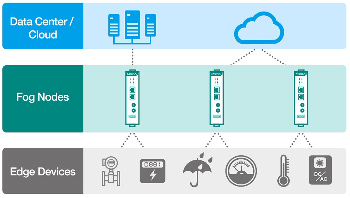
\includegraphics[width=.5\textwidth]{fig1.pdf}
    \caption [Organização arquitetural]
    {\label{fig:fig1} Organização arquitetural.} \cite{archfog:2017}
\end{figure}

Em uma abordagem \textit{bottom-up}, podemos descrever a arquiterura da computação em névoa como um conjunto de \textit{edge devices}\footnote{Dispositivo que controla o fluxo de dados no limite entre duas redes \cite{edgeDevices}.} que se comunicam com os \textit{fog nodes}, e esses com servidores centrais.
Entretanto, a comunicação entre os \textit{fog nodes} e os servidores centrais não é essencial para a execução dos serviços em névoa \cite{DBLP:journals/corr/RomanLM16}.
A Figura \ref{fig:fig1} representa este conceito de computação em névoa.

\section{Motivação e justificativa}

De acordo com Vaquero e Rodero-Merino \cite{Vaquero:2014}, serão sete os desafios que a computação em névoa deverá enfrentar para se tornar realidade.
Os problemas referentes à padronização, descoberta e sincronização são os motivadores deste trabalho, uma vez que atualmente não existem mecanismos
no qual um membro da rede, seja ele um dispositivo com limitações de memória e processamento ou um computador, mapeiem os recursos disponíveis e divulgue os seus na rede.

A ausência desses mecanismos faz com que cada membro interaja exclusivamente com seus recursos, portanto, não há compartilhamento entre os nodos da rede.
O motivo pelo qual os nodos não consomem os recursos de seus vizinhos está no desconhecimento dos mesmos, sendo assim, é inviável utilização de um recurso que não esteja atrelado ao próprio nodo.
Este compartilhamento de informações, referente aos nodos e recursos, justifica o desenvolvimento deste trabalho.


\section{Objetivo}

O objetivo principal deste trabalho de conclusão é resolver os desafios relacionados à padronização, descoberta e sincronização referidos por Vaquero e Rodero-Merino \cite{Vaquero:2014}.

Modelar e implementar um protocolo com baixo custo de transmissão, que seja distribuído, que se adeque a ambientes dinâmicos e que seja simples de ser
empregado em topologias de rede já implantadas são os objetivos desse trabalho. Dessa maneira, o processo de descoberta e sincronização de recursos ocorrerá de forma automatizada. %intro
  \chapter{\label{chap:chap2} Fundamentação Teórica}

Este capítulo apresentará alguns protocolos de comunicação e técnicas que servirão de apoio para o desenvolvimento deste TCC. 
Por fim, alguns trabalhos relacionados a área serão expostos, bem como o posicionamento deste trabalho perante aos demais.


\section{BGP}


O protocolo BGP está situado na quinta camada, a camada de aplicação, do modelo de referência TCP/IP \cite{tanenbaum2011redes}.
Abaixo, de forma sucinta, elencaremos algumas funcionalidades básicas do protocolo que embasarão o restante deste trabalho.

\begin{itemize}
    \item A responsabilidade deste protocolo é manter a troca de informações sobre roteamentos entre sistemas autônomos \cite{Rekhter:1995}.
    \item O roteador ao entrar na rede pela primeira vez deve-se conectar ao seu vizinho. Após a conexão estabelecida, os roteadores compartilham entre sí suas tabelas de roteamento \cite{Rekhter:1995}.
    \item Posteriormente, as atualizações nas tabelas dos roteadores dão-se de forma incremental à medida que as mudanças na rotas ocorrem \cite{Rekhter:1995}.
    \item Mensagens de \textit{keep alive} são trocadas periodicamente a fim de garantir conectividade entre os roteadores \cite{Rekhter:1995}.
\end{itemize}

\section{CoAP}

Especificado pela RFC-7252, o CoAP, protocolo de aplicação restrita, foi projetado para aplicações máquina-a-máquina
e tem como foco a transferência de documentos web entre nodos com recursos limitados em redes de baixa qualidade\cite{rfc7252}.

% falar do service discovery e resource directory.

O modelo de interação cliente/servidor é o padrão adotado pelo CoAP, entretanto,
o fato do protocolo ter sido projetado para aplicações máquina-a-máquina faz com que os dispositivos comumente desempenhem o papel de cliente e servidor simultaneamente.

Quando mensagens CoAP de requisição e resposta são trocadas, estas devem conter o código do método ou código da resposta, respectivamente.
Além dos códigos, as mensagens podem conter outras informações, como o recurso que se deseja acessar e o tipo de mídia que se está transportando.
Por fim, um token é utilizado para que haja a correspondência entre requisição e resposta.

A Figura \ref{fig:fig4} ilustra uma solicitação entre cliente e servidor, na qual o cliente deseja obter a temperatura.
Analisando a troca de mensagens, notamos que o cliente envia uma solicitação não confirmável com token 0x74 e código GET para acessar o recurso temperatura no servidor.
O servidor por sua vez retorna o código de resposta 2.05, que indica sucesso, o mesmo token que recebeu na solicitação do cliente e o valor 22.5 C.


\begin{figure}[htb!]
    \centering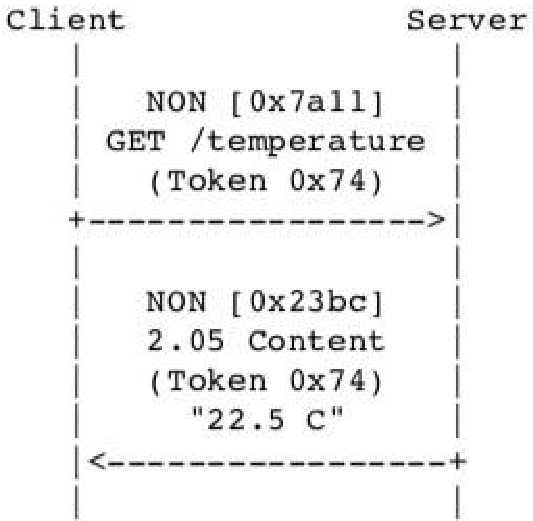
\includegraphics[height=.5\textwidth]{fig4.pdf}
    \caption
    {\label{fig:fig4} Requisição e resposta utilizando mensagens não confirmáveis.} \cite{rfc7252}
\end{figure}

A arquitetura REST, assim como no protocolo HTTP\cite{rfc2616}, foi utilizada na projetização do protocolo CoAP.
Como ambos compartilham da mesma arquitetura, realizar o mapeamento de HTTP para CoAP e vice-versa é bastante simples.
Para realizar tal mapeamento basta utilizarmos o cross-proxy, definido na sessão 10 da própria RFC-7252\cite{rfc7252},
que converte o método ou tipo de resposta, tipo de mídia e opções para os valores HTTP correspondentes.

Além de modelo de comunicação cliente/servidor e arquitetura REST, o CoAP também dispõem de outros princípios comuns ao HTTP e que são conceitos padrão na web
como suporte a URIs\cite{rfc3986} e tipos de mídia da Internet(MIME)\cite{rfc2046}.

Entre o HTTP e CoaP nem tudo são semelhanças, pois, obviamente, este possui particularidades para que consiga atender aos requisitos no qual se propõe a resolver.
Entre as diferenças está a troca de mensagens assíncronas utilizando transporte orientado a datagramas, como UDP.
Apesar de, naturalmente, o protocolo UDP não prover confiabilidade, no CoAP é possível definir que as mensagens possuam tal aspecto.
CoAP-URI schema e service discovery, que serão abordados nas sessões a seguir, possibilidade de envio de solicitacoes multicast e unicast, cabeçalho com baixa sobrecarga de dados e segurança na forma de DTLS\cite{rfc6347}
estão entre as principais caracteristicas do protocolo de aplicação restrita, CoAP.

\section{CoAP - URIs }

De forma análoga ao HTTP  e o HTTPS, o protocolo CoAP provê suporte aos esquemas do tipo \textit{coap} e \textit{coaps}, este utilizando segurança DTLS.
Estes esquemas são utilizados para identificar e localizar os recursos coap na rede.
Portanto, servidores coap ficam aguardando por requisições que utilizem tal esquema.

A definição sintática, segundo Backus-Naur Form RFC-5234\cite{rfc5234},  do  CoAP-URI está definida abaixo:

\begin{verbatim}
    CoAP-URI = "coap:" "//" host [ ":" port ] path-abempty [ "?" query ]
\end{verbatim}

O esquema CoAP-URI suporta o prefixo \textit{/.well-known/} , definido na RFC-5785\cite{rfc5785}.
Este prefixo é utilizado para que o servidor exponha suas políticas e recursos disponíveis.

O exemplo abaixa demostra um fluxo de requisição e resposta utilizando o prefixo \textit{/.well-known/}.

\begin{verbatim}
    REQ: GET coap://example.net/.well-known/core
\end{verbatim}

\begin{verbatim}
    RES: 2.05 Content
    </sensors/temp>;if="sensor",
    </sensors/light>;if="sensor"
\end{verbatim}

Notamos, então, que o servidor nomeado example.net possui os recursos \textit{temp} e \textit{light} disponíveis para serem utilizados através do protocolo coap.


\section{Trabalhos Relacionados}

% iotivity

Spencer Lewson implementou um protocolo em nível de aplicação \cite{tanenbaum2011redes} capaz de realizar a comunicação entre nodos sob computação em névoa.
A especificação do protocolo e um \textit{middleware}, capaz de realizar o gerenciamento dos recursos dos dispositivos, são os principais componentes deste trabalho \cite{Spencer:2015}.

Sua implementação requer que haja um ponto central de comunicação entre os nodos, uma vez que a conectividade entre eles ocorre via \textit{Bluetooth LE}.
A existência desse ponto justifica-se pelas regras de implementação do \textit{Bluetooth LE}, na qual descreve dispositivos de duas naturezas: centrais e periféricos.
Dispositivos centrais são responsáveis por descobrir dispositivos periféricos que estão interessados em criar conexão.
Portanto, a característica do \textit{Bluetooth LE} faz com que a topologia de rede e a arquitetura do projeto não seja distribuída \cite{Spencer:2015}.





 %ref teorico. estado da arte
  \chapter{\label{chap:chap3} Projeto}



A organização e a descrição deste projeto serão apresentados neste capítulo.
Para tal, nas seções a seguir abordaremos a arquitetura, o formato de mensagens, módulos e submódulos que o constituem.

\section { Arquitetura }

Seguindo a topologia da Figura \ref{fig:fig14}, podemos observar que os \textit{fog nodes} não possuem um nodo central como servidor.
Sendo assim, os fog nodes e os edge devices comunicam-se utilizando o protocolo CoAP.
Dessa maneira, as Requisições entre fog nodes só ocorre caso o nodo requisitante saiba, previamente, o endereço IP relativo ao nodo solicitado.

\begin{figure}[H]
    \centering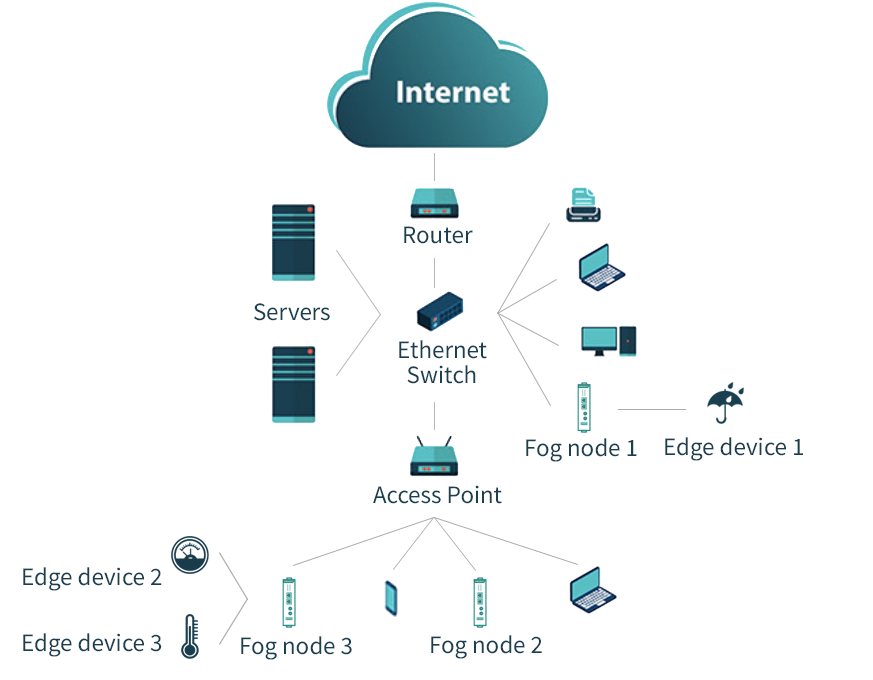
\includegraphics[width=.8\textwidth]{fig14.png}
    \caption [Topologia LAN]
    {\label{fig:fig14} Topologia LAN.}
\end{figure}

Em razão da topologia distribuída, a arquitetura deve ser capaz de mapear e sincronizar, de forma autônoma, os recursos providos pelos fog nodes.
Dessa forma, cada \textit{fog node} saberá quais são os \textit{edge devices} disponíveis na rede, portanto,
o nodo que possui o sensor de chuva saberia que existe um outro nodo em sua LAN capaz de medir a temperatura, por exemplo.

A arquitetura proposta, no que se refere a comunicação entre fog nodes e edge devices, utilizou como base um fork da implementação do protocolo CoAP\cite{coapimpl:2018}.
Esse fork, implementado em Python e de acordo com a RFC-7252, consiste em dois grandes módulos: \textit{CoAP-Server} e \textit{CoAP-Client}.
O primeiro, é responsável pelo recebimento das Requisições, e foi alterado com o objetivo de proporcionar o dinamismo na inserção e remoção dos recursos sem a necessidade de sua reinicialização.
O segundo módulo é encarregado de realizar as Requisições diretamente aos nodos, e para essa funcionalidade nenhuma alteração no projeto original foi realizada.


Observando a Figura \ref{fig:fig15}, podemos notar que a arquitetura de um fog node é composta por três grandes camadas, sendo elas hardware, sistema operacional e aplicações.

Na camada de hardware podemos utilizar desde um dispositivo com limitações de memória e CPU até um aparelho com grande capacidade computacional.
Já na camada de sistema operacional, temos a liberdade de utilizar uma vasta diversidade de distribuições Unix.
Por fim, na camada de aplicação devemos executar os processos \textit{CoAP-Server}, \textit{CoAP-Client} e \textit{Resource-Mapping}.

\begin{figure}[H]
    \centering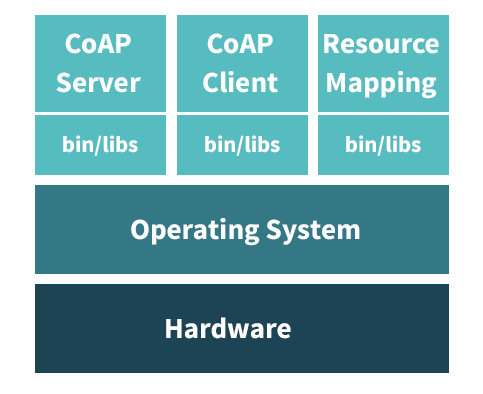
\includegraphics[width=.5\textwidth]{fig15.png}
    \caption[Arquitetura de um fog node]
    {\label{fig:fig15} Arquitetura de um fog node.}
\end{figure}

A Figura \ref{fig:fig16} exibe, de maneira detalhada, os processos envolvidos na execução no protocolo \textit{Resource-Mapping}.
Nela podemos destacar a presença de três entidades principais, \textit{Observer}, \textit{Keep Alive} e \textit{Receptor}.
Abaixo elencaremos as funcionalidades de cada entidade.

\begin{itemize}
    \item \textit{Observer} é responsável por manter o estado de seus proprios recursos atualizados.
    \item \textit{Keep Alive} tem a missão de manter seus vizinhos de rede atualizados sobre seu estado de operação.
    \item \textit{Receptor} é incumbido de receber e processar as requições recebidas via \textit{Resource-Mapping}.
\end{itemize}

\begin{figure}[H]
    \centering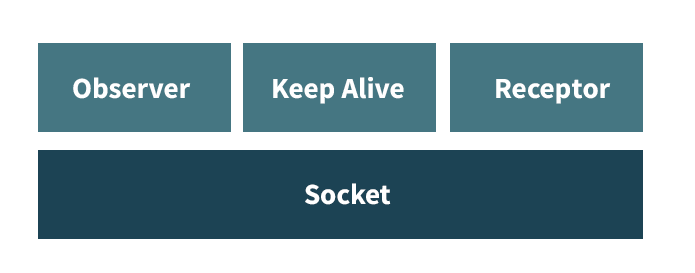
\includegraphics[width=.5\textwidth]{fig16.png}
    \caption[Arquitetura Resource-Mapping]
    {\label{fig:fig16} Arquitetura Resource-Mapping.}
\end{figure}


\section{Requisitos e limitações}

Para que a solução opere corretamente, tanto no mapeamento quanto na sincronização de recursos, algumas limitações e requisitos necessitam ser expostas.

Como proposição inicial temos que o sistema operacional deve ser Unix e o usuário corrente deve dispor de privilégios de root.
Além disso, a linguagem de programação Python em sua versão 2.7 com seu respectivo gerenciador de pacotes, \textit{PIP}\cite{pip}, devem estar instalados.
Por fim, os dados que os edge devices fornecerão aos fog nodes serão tratados de forma simulada, pois o funcionamento exato dos sensores e atuadores
fogem do escopo desse projeto. As Seções 4.3.1 e 4.3.2 utilizarão essas simulações a fim de validar o protocolo.


\section{Formato de mensagens}

Esta Seção define a pilha de protocolos a serem utilizados neste projeto, a justificativa pelas suas escolhas, e por fim, o detalhamento do protocolo proposto.
A pilha de protocolos atuará em conjunto com a organização arquitetural previamente definida na Figura \ref{fig:fig1}.

A fim de facilitar a compreensão da arquitetura deste projeto, a Figura \ref{fig:fig2} explicita a pilha de protocolos que o projeto fará uso para implementar as funcionalidades propostas.

\begin{figure}[htb!]
    \centering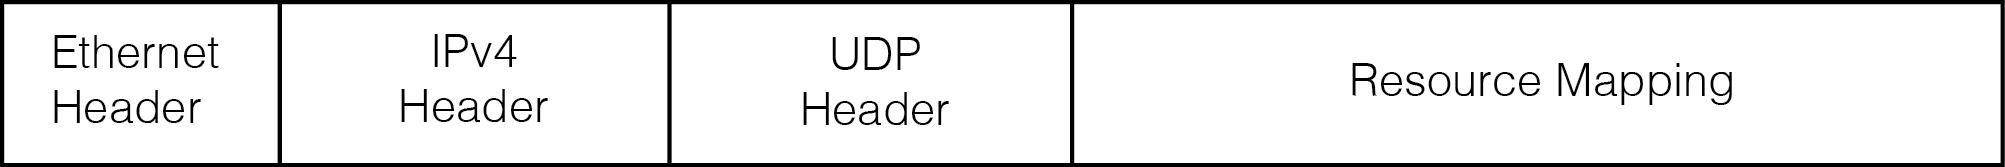
\includegraphics[width=.8\textwidth]{fig2.png}
    \caption[Pilha de protocolos]
    {\label{fig:fig2} Pilha de protocolos.}
\end{figure}

O modelo de referência TCP/IP é constituido de cinco camadas: física, enlace, rede, transporte e aplicação \cite{tanenbaum2011redes}.
Nesse trabalho, o níveis de rede e transporte (IPv4 e UDP respectivamente) serão utilizados para a implementação do modelo proposto.

A utilização de IPv4 na camada de rede justifica-se pelo fato do protocolo ser empregado em redes locais, que geralmente não necessitam de uma quantidade de endereçamento tão grande 
se comparado ao IPv6, mas não existem impedimentos para que implementações futuras utilizem IPv6 na camada de rede.

Manter o contexto de conexão entre os nodos, utilizando TCP por exemplo, despenderia uma quantidade de trafego desnecessário na rede.
Visto que o baixo custo na transmissão de dados é um dos objetivos desse trabalho, a utilização de datagramas UDP faz sentido para que a se aumente o desempenho da solução.

A Figura \ref{fig:fig12} apresenta, de forma detalhada, a estrutura dos dados contidos no protocolo \textit{Resource Mapping}.

\begin{figure}[htb!]
    \centering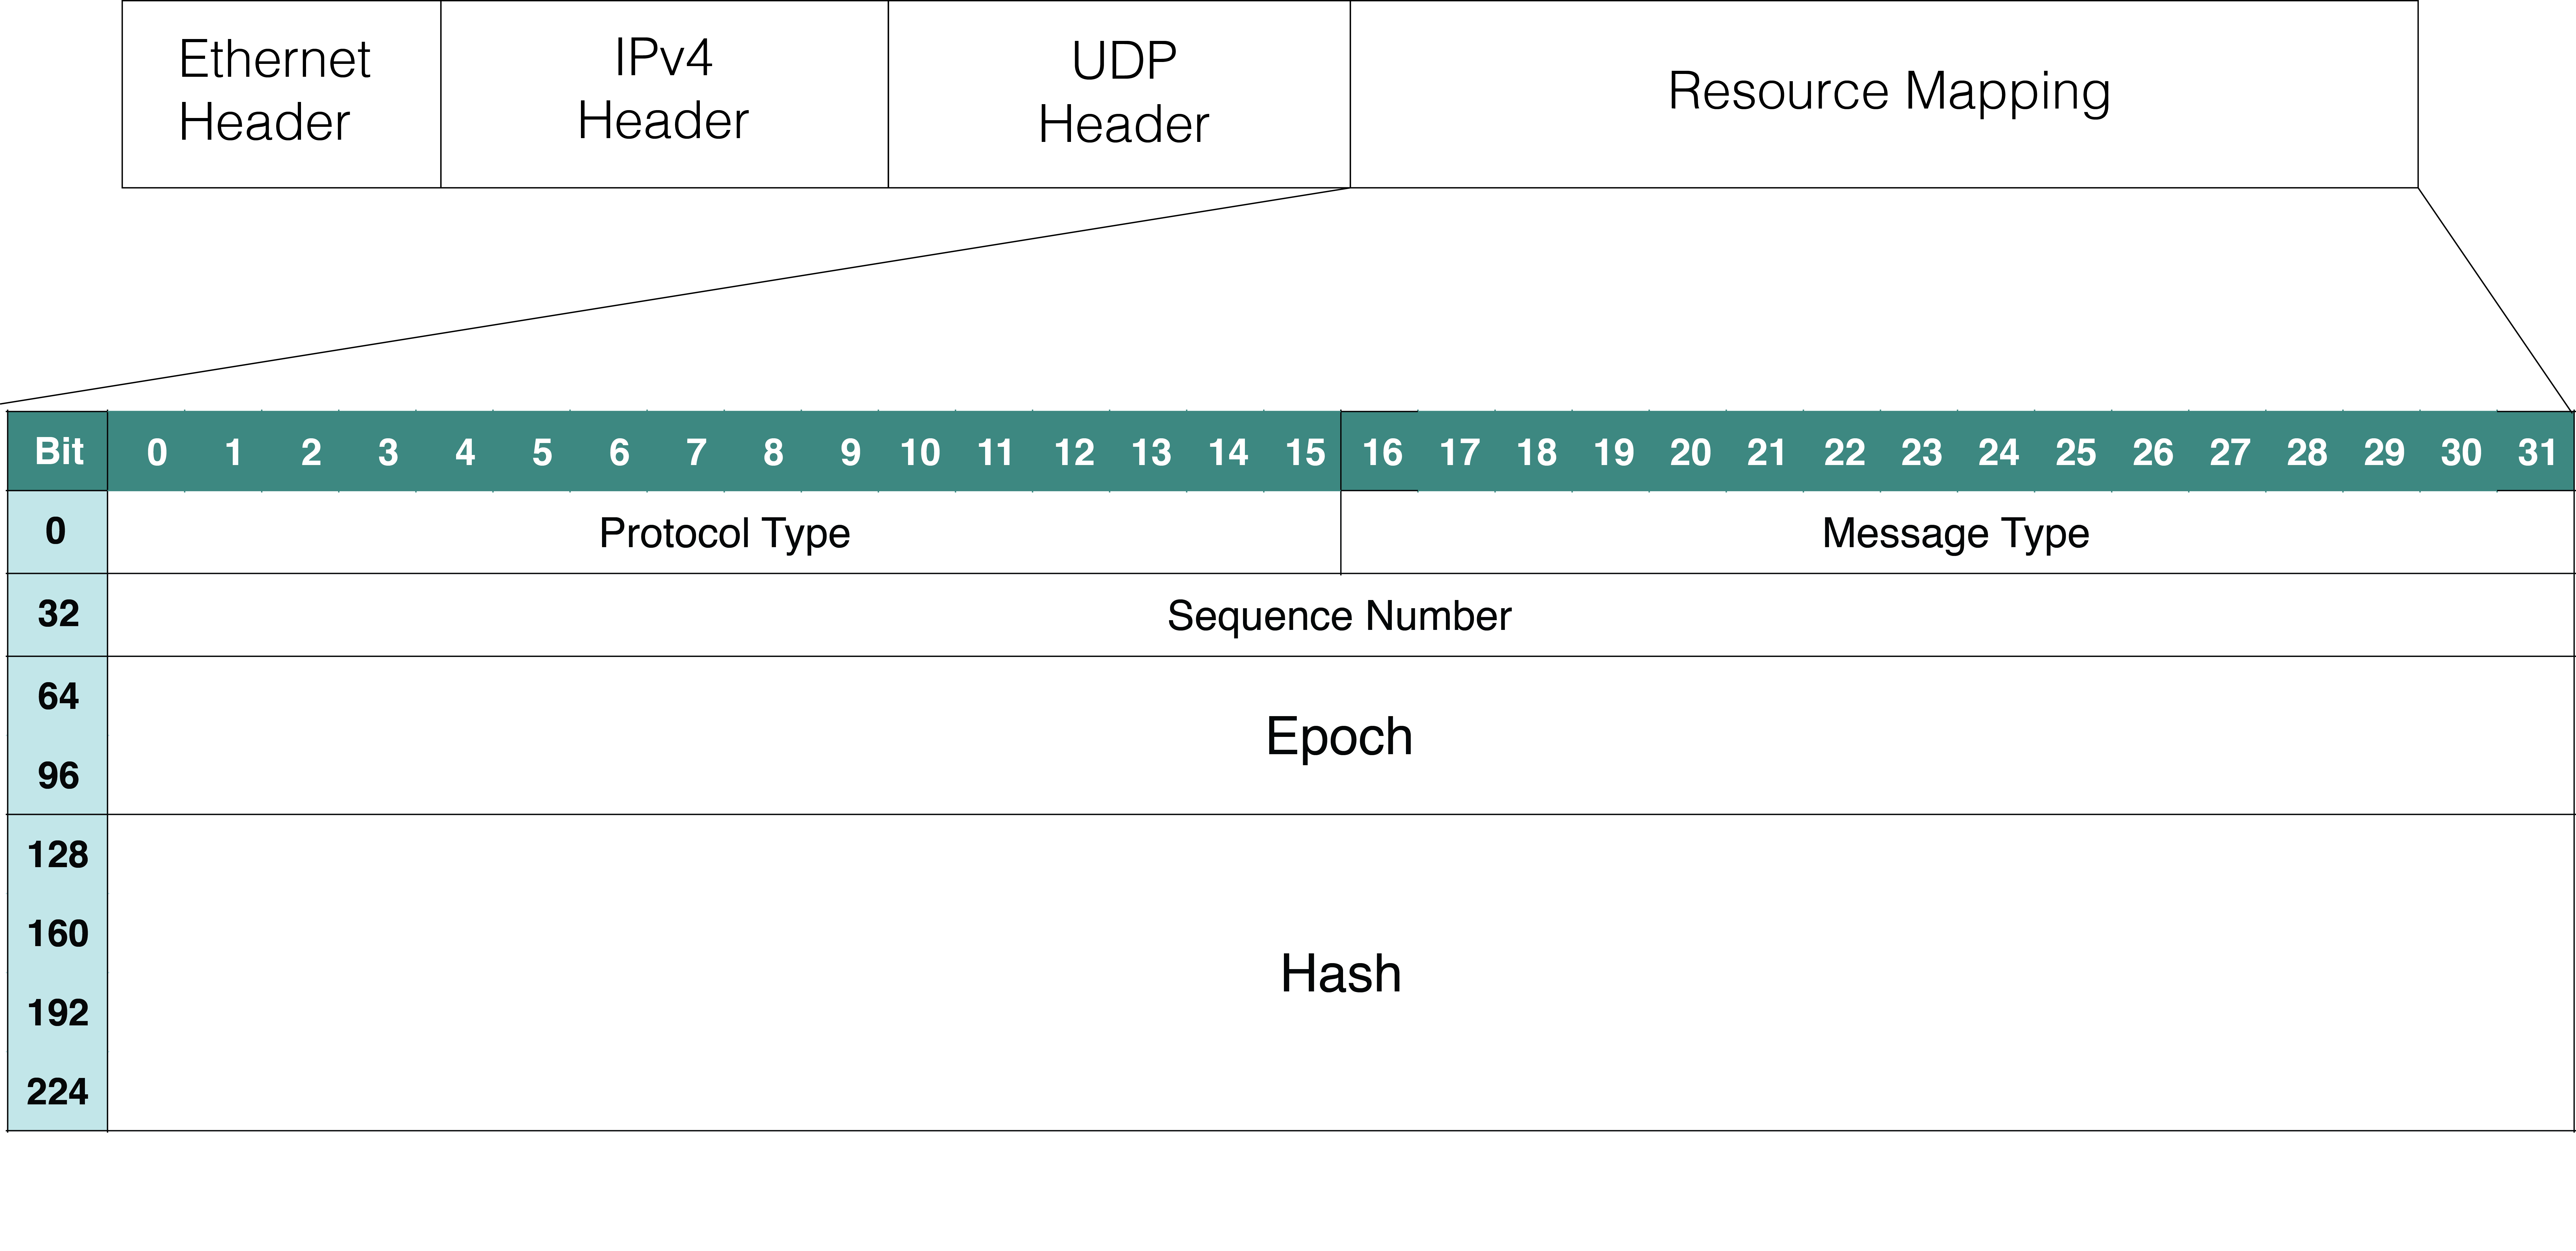
\includegraphics[width=.8\textwidth]{fig12.png}
    \caption[Detalhamento Resource Mapping]
    {\label{fig:fig12} Detalhamento Resource Mapping.}
\end{figure}

\begin{itemize}
\item O campo Protocol Type é reservado para indicar a forma de encapsulamento do pacote.
Dessa forma, o restante dos campos do pacote podem ser tratados de acordo com a definição dada pelo campo.
\item Atualmente existem dois tipos de Messages Types possíveis, keep alive e acknowledgement.
\item Sequence Number tem o intuito de identificar o pacote enviado.
\item O campo Epoch é utilizado para indicar alterações nos recursos providos pelo fog node.
Sendo assim, quando um recurso é adicionado ou removido de um fog node, o campo Epoch é acrescido em uma unidade. Os detalhes de seu comportamento serão abordados na Seção 3.3.2.
\item O campo Hash utiliza a função de criptografia MD5 para validar a integridade dos demais campos contidos no pacote.
\end{itemize}

O protocolo proposto, intitulado \textit{Resource Mapping}, como apresentado nas Figuras \ref{fig:fig2} e \ref{fig:fig12}, atuará na camada de aplicação do modelo de referência TCP/IP \cite{tanenbaum2011redes} e será responsável por padronizar, descobrir e sincronizar os nodos da névoa.
Os maiores desafios neste modelo proposto são manter o estado global dos recursos acessível a todos os nodos, e garantir que o desempenho seja satisfatório com o objetivo permitir a escalabilidade da solução.


\section{Módulos}

De forma geral, cada nodo da rede mantém uma lista com os endereços IP`s que fazem parte do mapeamento.
Atrelado à cada endereço IP,  há uma lista com os recursos providos por este.
Em vista disso, cada nodo contém um mapeamento global de recursos disponíveis na névoa.

O detalhamento das funcionalides que o projeto possui, tal como ilustrações relacionadas aos fluxos, serão abordadas nas proximas subseções.

\subsection{Descoberta de recursos}


Partindo do pressuposto que os nodos da névoa já possuem seus recursos devidamente criados e acessíveis via CoAP,
como primeiro passo do mapeamento devemos considerar a entrada de um novo nodo na rede.
No momento em que o nodo dispor de um endereço IP válido, este deverá enviar um pacote para o endereço de multicast indicando que possui recursos a serem disponibilizados.


Ao receberem o pacote enviado por multicast, os nodos que desejarem saber quais recursos estão sendo providos por este novo membro, deverão realizar uma Requisição
unicast para a URI \textit{/.well-known/core} utilizando o protocolo CoAP.
Vale lembrar que este fluxo de requisição e resposta, utilizando a URI \textit{/.well-known/core}, faz com que o nodo requisitado retorne todos seus recursos ao solicitante.

\begin{figure}[H]
    \centering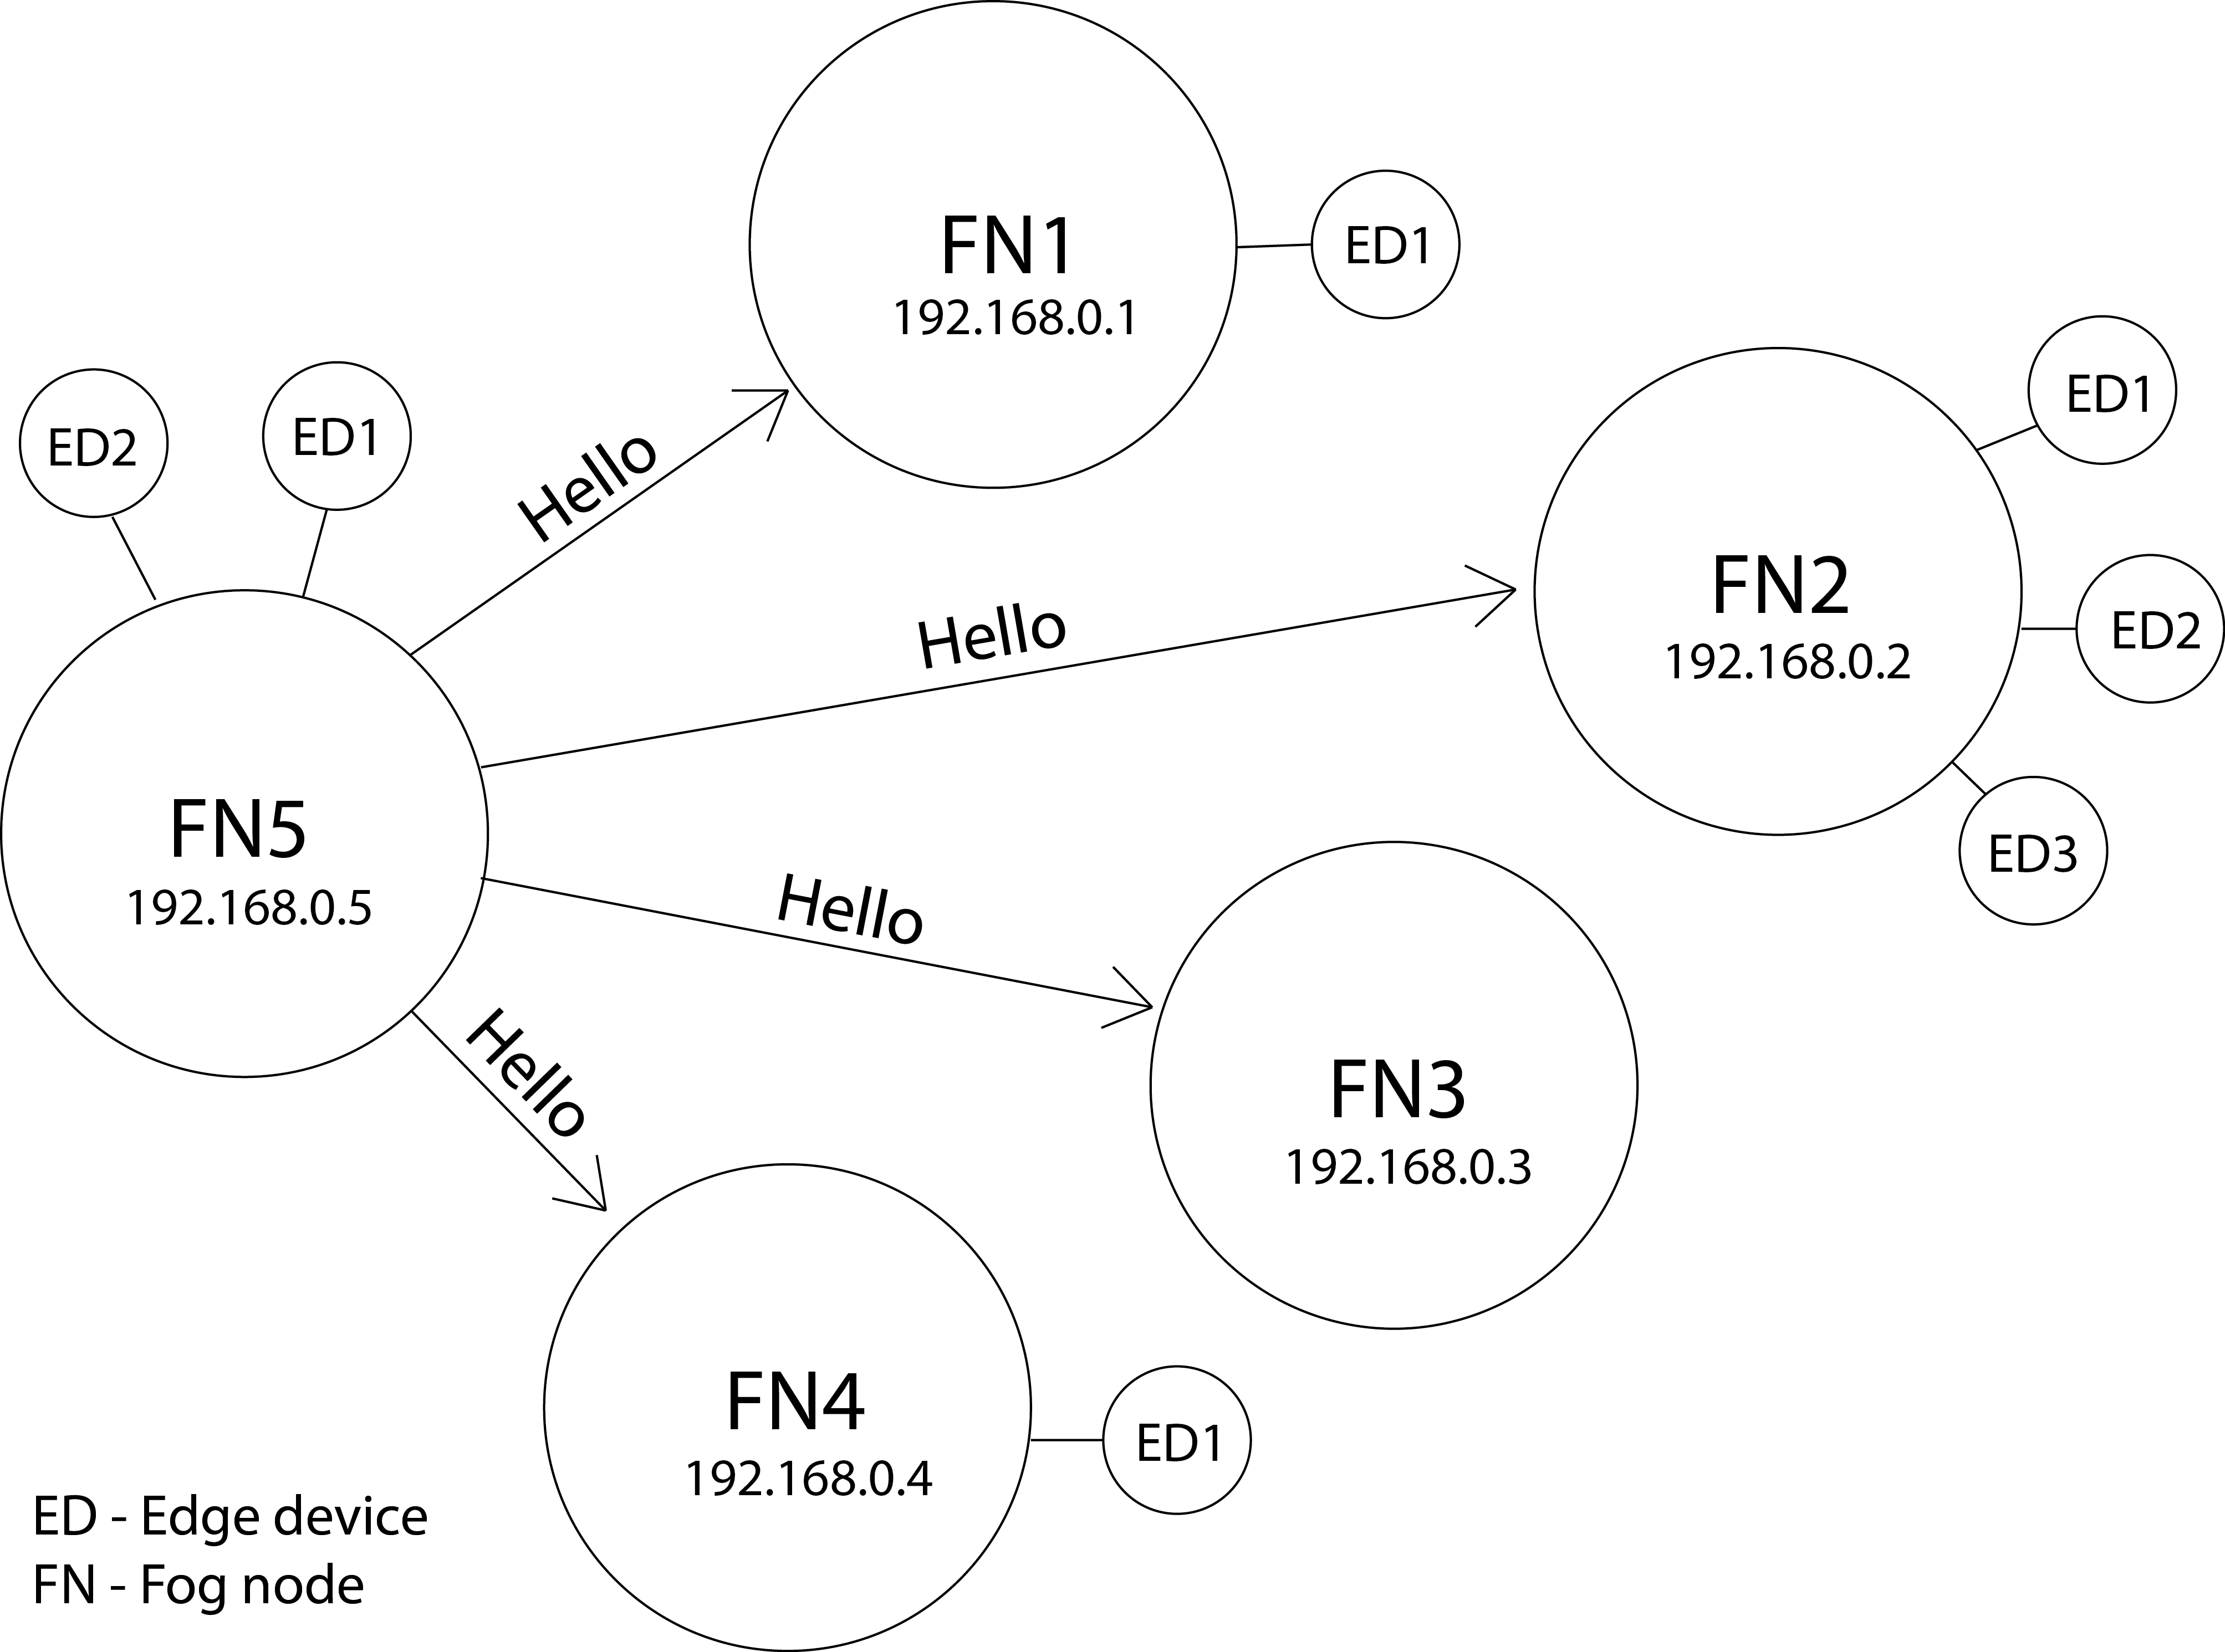
\includegraphics[width=.8\textwidth]{fig5.png}
    \caption[Nodo entrando na névoa]
    {\label{fig:fig5} Nodo entrando na névoa.}
\end{figure}

A topologia da névoa utilizada nas Figuras \ref{fig:fig5} e \ref{fig:fig6} é definida por fog nodes enumerados de um a cinco, sendo o nodo FN5 o último a entrar na rede.
A figura \ref{fig:fig5} demonstra o nodo FN5 entrando na névoa e, portanto, deverá anunciar-se por multicast indicando que possui recursos a serem disponibilizados.

Após FN5 enviar mensagem de Olá por multicast, os nodos FN1, FN2 e FN4 realizam a Requisição CoAP diretamente ao FN5 afim de obter os recursos disponíbilizados por ele,
já o nodo FN3, por não estar executando o protocolo de mapeamento, não realiza a Requisição CoAP.

\begin{figure}[H]
    \centering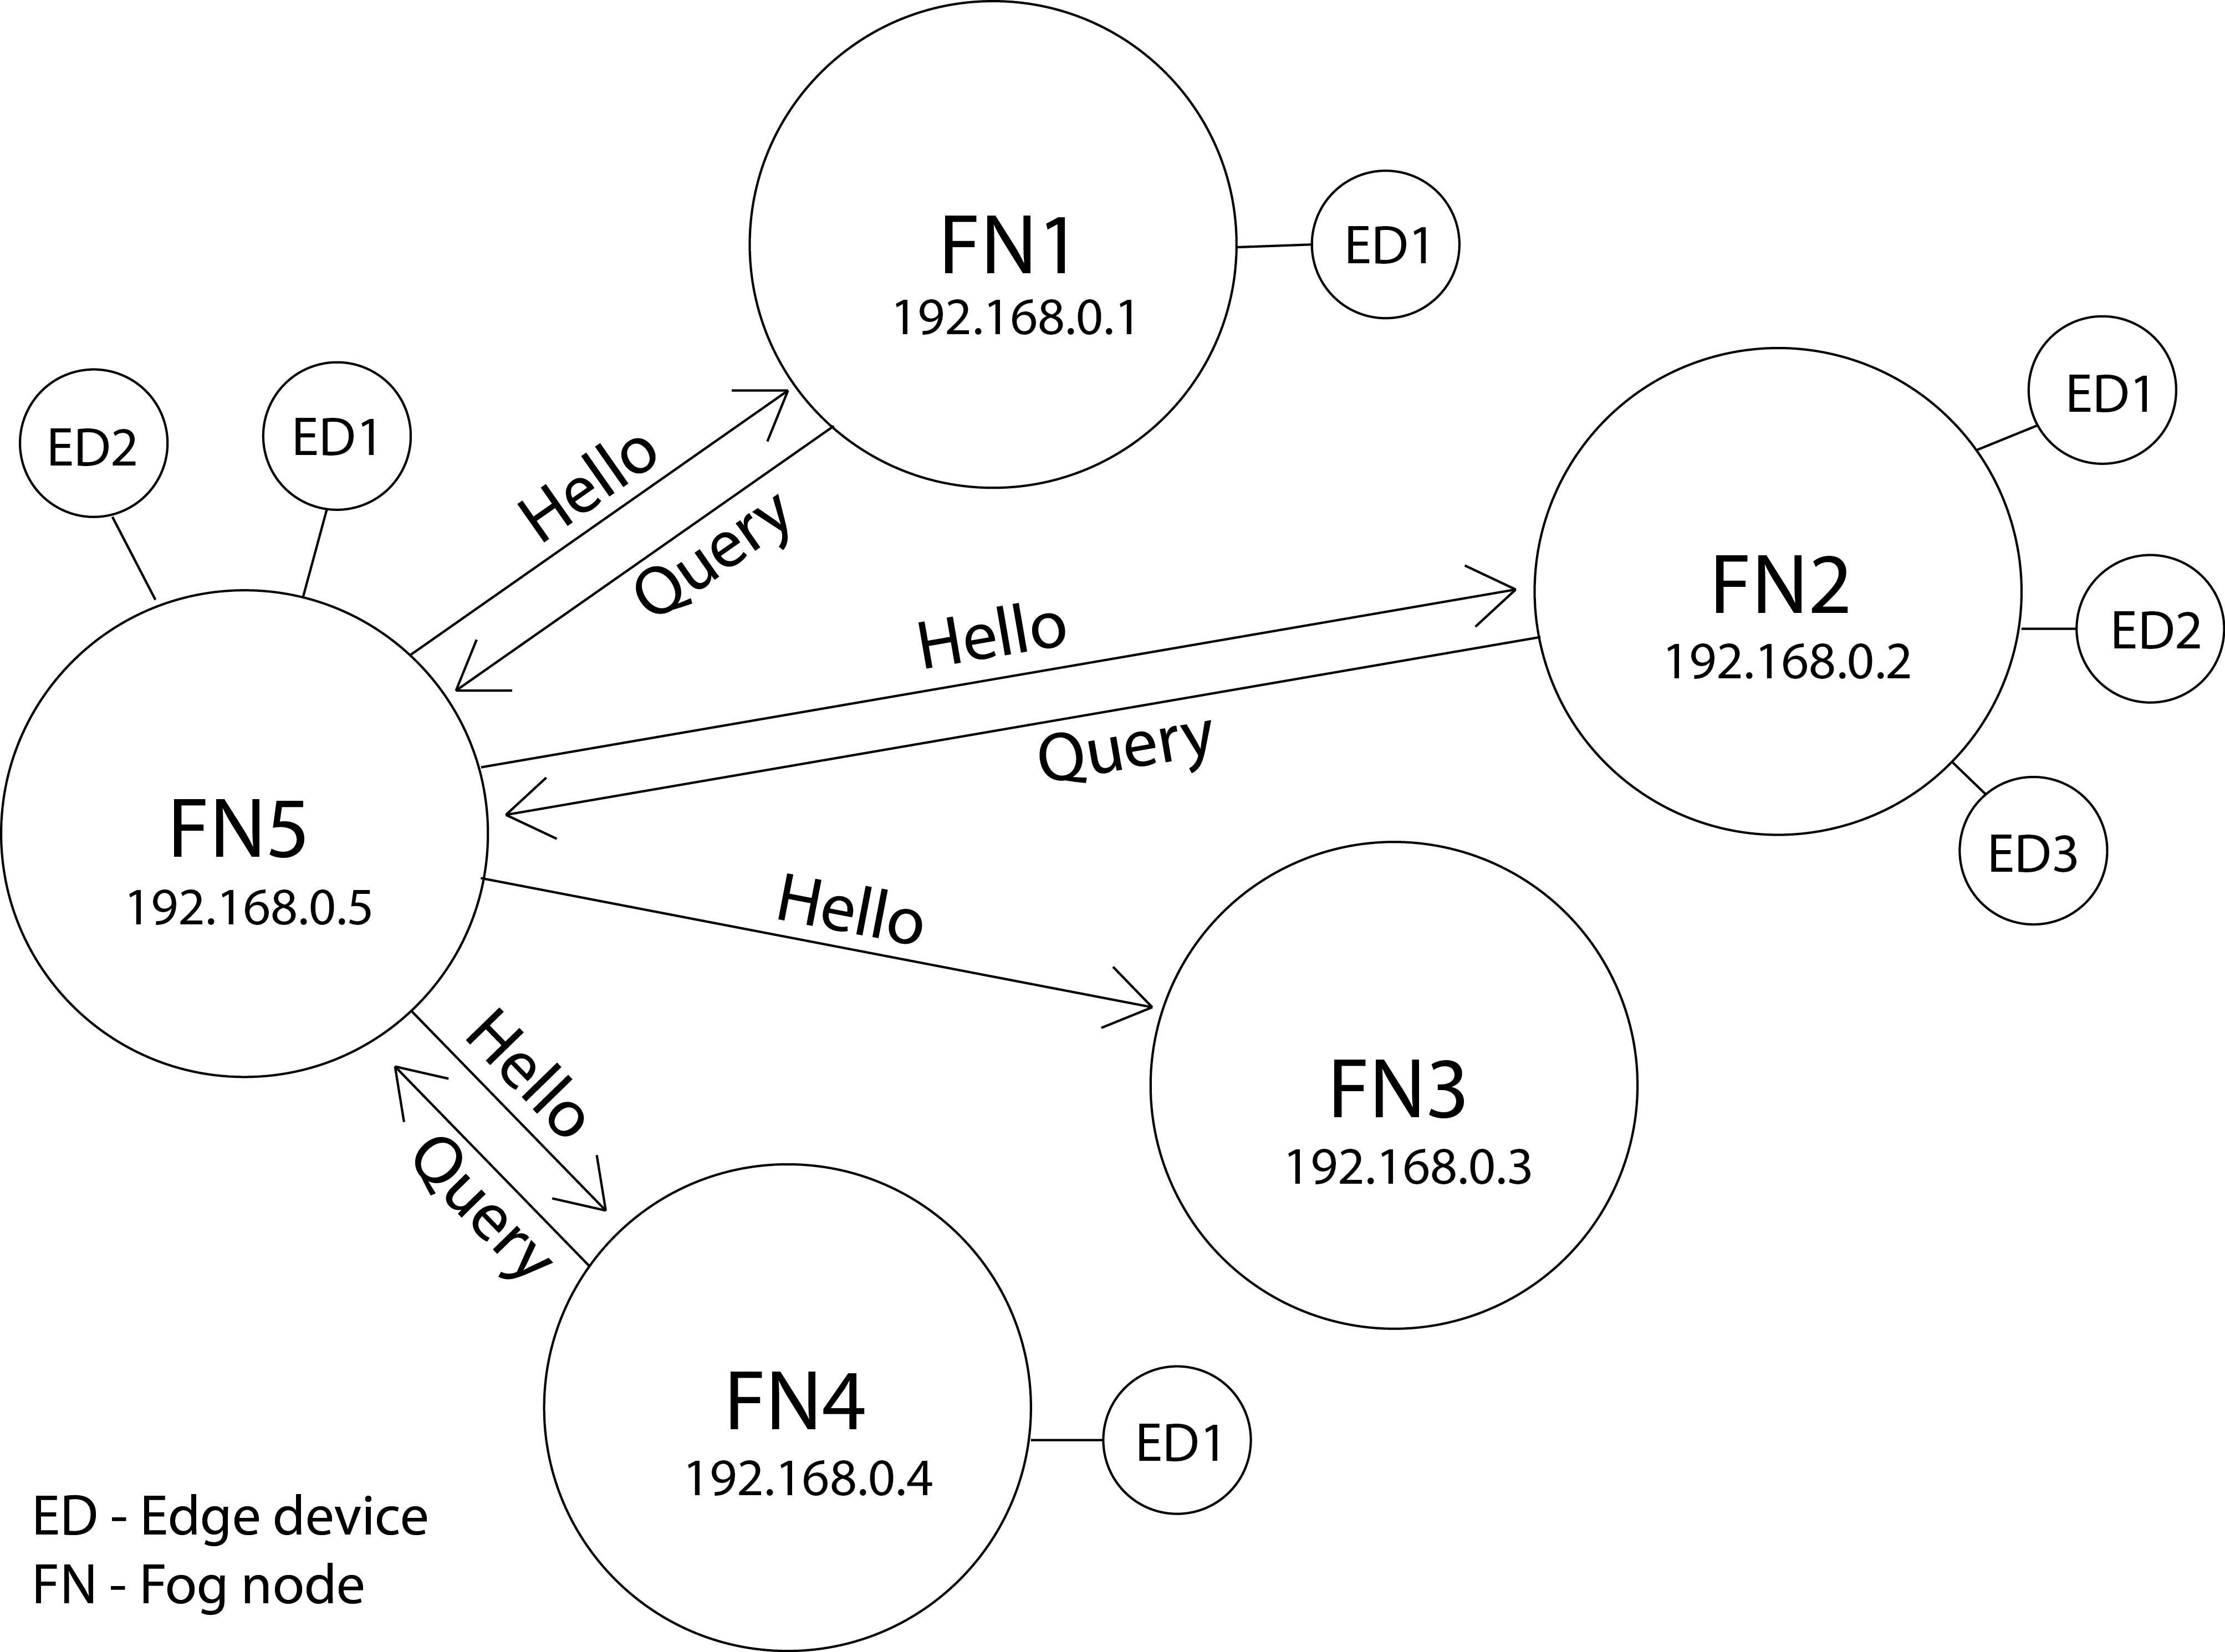
\includegraphics[width=.8\textwidth]{fig6.png}
    \caption [Requisição entre fog nodes]
    {\label{fig:fig6} Requisição entre fog nodes.}
\end{figure}


\subsection{Gerenciamento de recursos}

A manutenibilidade da lista de recursos globais é relevante para que o protocolo funcione de acordo com a especificação, pois, a névoa deverá saber quando um nodo, ou recurso dele, deixou de fazer parte da rede.
Para tal, faz-se necessário a utilização de alguns mecanismos de controle.
Esses controles são realizados em duas esferas, a primeira trata da inserção ou remoção de um nodo na rede,
já a segunda refere-se a inserção ou remoção de um edge device vinculado a um nodo qualquer.


Inicialmente abordaremos a entrada e saída de nodos da névoa, e para esta subseção será utilizado o cenário da Figura \ref{fig:fig6} quando necessário.
O Pseudocódigo \ref{alg:alg1} demonstra, de forma sucinta, a política de atualização que cada nodo deverá implementar no recebimento de mensagens de keep alive.


\begin{algorithm}[H]
    \begin{center}
        \begin{algorithmic}[1]
            \STATE \textbf{function} $\text{Policy(ip, epoch, myEpoch)}$
            \STATE \hspace{\algorithmicindent} \textbf{if} $\text{exists(ip)}$
            \STATE \hspace{\algorithmicindent} \hspace{\algorithmicindent} \textbf{if} $\text{epochHasChanged(epoch, myEpoch)};$
            \STATE \hspace{\algorithmicindent} \hspace{\algorithmicindent} \hspace{\algorithmicindent} $\text{resources = getResourcesCoAP(ip, '/.well-known/core')};$
            \STATE \hspace{\algorithmicindent} \hspace{\algorithmicindent} \hspace{\algorithmicindent} $\text{update(ip, resources)};$
            \STATE \hspace{\algorithmicindent} \textbf{else}
            \STATE \hspace{\algorithmicindent} \hspace{\algorithmicindent} $\text{resources = getResourcesCoAP(ip, '/.well-known/core')};$
            \STATE \hspace{\algorithmicindent} \hspace{\algorithmicindent} $\text{insert(ip, resources)};$
            \STATE \hspace{\algorithmicindent} $\text{sendAcknowledgement(ip)};$

        \end{algorithmic}
    \end{center}
    \caption[Política de atualização de recursos]%
        {\label{alg:alg1} Política de atualização de recursos.}%
    \end{algorithm}

No momento em que o nodo recebe a resposta da chamada de função \textit{getResourcesCoAP}, contendo os recursos providos pelo nodo requisitado, aquele deverá armazenar as informações em uma estrutura de dados adequada.
Essa estrutura de dados estará implementada em todos os nodos da névoa, e a partir dela será possível realizar o gerenciamento dos recursos de forma simples e eficiente.
O trecho abaixo define, por ora, o formato dos dados que serão utilizados em cada nodo.


\begin{verbatim}
    Fog = {
        string ip;
        string resources[];    
    };
    Fog fogs[];
    string myResources[];
\end{verbatim}

De posse da Figura \ref{fig:fig6} como cenário, do algoritmo de atualização \ref{alg:alg1}, e da estrutura de dados previamente descrita,
demonstramos abaixo o estado em que se encontram os dados armazenados em FN2 após a aplicação do método.

\begin{verbatim}
    fogs: [
        {
            ip: '192.168.0.1',
            resources: [ 'ED1' ]
        },
        {
            ip: '192.168.0.3',
            resources: [ ]
        },
        {
            ip: '192.168.0.4',
            resources: [ 'ED1' ]
        },
        {
            ip: '192.168.0.5',
            resources: [ 'ED1', 'ED2' ]
        }
    ];
    myResources: [ 'ED1', 'ED2', 'ED3' ];
\end{verbatim}

Visto isso, é imprescindível que os nodos mantenham seus dados consistentes, pois, após adicionar o novo nodo em sua lista de fogs, o protocolo precisa ser capaz de perceber quando um elemento
deixou de fazer parte do processo. Assim, a manutenção dos estados será abordado de forma similar as mensagens de \textit{keep alive} utilizadas no protocolo BGP\cite{Rekhter:1995}.
Mensagens de keep alive são adotadas para que os nodos da rede avisem seus vizinhos que ainda estão em operação, pois, sem esse procedimento seria difícil
saber quando remover um IP da lista de recursos. Portanto, para manter a lista atualizada, este protocolo implementa mensagens desse tipo.

As mensagens de keep alive serão transmitidas sob multicast em um intervalo de trinta segundos, porém, este é apenas um valor arbitrário, e pode ser alterado
para que a solução obtenha uma melhor eficiência.
Após o recebimento da mensagem de keep alive, os nodos deverão respondê-las indicando que ainda estão em operação.
Caso o nodo não responda a mensagem de keep alive, este será marcado como parcialmente inativo pelo remetente da mensagem.
Quando o nodo solicitante realizar outra mensagem de keep alive e o nodo que já estava marcado com parcialmente inativo não responder, o mesmo será removido da lista de recursos do
solicitante, e assim é possível saber quando um nodo deixou de fazer parte da névoa.
Para realizar este controle será preciso adicionar na estrutura \textit{Fog} a propriedade boleana, denominada \textit{isReplyingKeepAlive}, que indica se o nodo está respondendo a solicitações de keep alive.

As mensagens de keep alive mantém os nodos informados sobre o estado de seus vizinhos, mas não conseguem indicar informações relacionadas aos edge device.
Consequentemente, não é possível saber quando um edge device parou ou iniciou sua operação em um nodo ativo.

Para que seja possível detectar esse tipo de comportamento, o protocolo proposto deverá implementar a técnica denominada \textit{época},
e servirá para que os nodos mantenham ciênia sobre o estado dos edge devices de seus vizinhos de rede.
Para isso, uma nova propriedade denominada \textit{epoch}, do tipo inteiro, deverá ser adicionada a estrutura de dados, e estará presente tanto no nodo em si quanto em cada item da lista de fogs.
O valor da \textit{epoch} será incrementado em uma unidadade a toda alteração observada no nodo, seja pelo acréscimo ou pela remoção de edge devices.

Esta observação atuará realizando requisições para a URI /.well-known/core no endereço de loopback do próprio nodo,
assim, obterá seus recursos disponíveis e poderá comparar com os que possui armazenado em sua estrutura de dados.
Havendo divergências, como mencionado anteriormente, a propriedade época será incrementada em uma unidadade.

A partir de agora, então, todas as mensagens de keep alive deverão conter a época do nodo que está realizando o multicast.
Assim, todo nodo que receber a mensagem poderá comparar a época recebida na mensagem com a época que possui armazenada em sua lista de fogs referente ao remetente da mensagen.
Havendo divergência de épocas, este deverá realizar uma nova requisição para atualizar sua lista de recursos referente aquele nodo em específico.

Após as alterações realizadas na estrutura de dados, abaixo temos o novo modelo que suportará as funcionalidades propostas.
\begin{verbatim}
    Fog = {
        string ip;
        string resources[];
        int epoch;
        boolean isReplyingKeepAlive;
    }
    Fog fogs[];
    string myResources[];
    int epoch;
\end{verbatim} %proposta
  \chapter{\label{chap:chap4} Ambiente de simulação e estudos de caso}
% Sérgio: Este capítulo poderia se chamar "Ambiente de simulação e estudos de caso"

\section{Ambiente de simulação}
% Seção: "Ambiente de simulação" - descrever como tu montou tuas simulações, e como foi organizado o ambiente, etc..
Em um primeiro momento a névoa foi construída de forma simulada utilizando a ferramenta Common Open Research Emulator (CORE)\cite{coregui}.
Para os primeiros experimentos a ferramente obteve resultados satisfatórios, porém quando foi necessário escalarmos a solução ela se mostrou ineficiente.
A ineficiência estava na criação dos nodos e na execução dos protocolos CoAP e Resource Mapping, uma vez que eles deveriam ser executados em todos os hosts da rede e não havia 
meios de automatizar este processo.

Esta automatização foi implantada utilizando a SDK de gerenciamento de containers Docker para Python, desta forma, foi possível criarmos névoas com tamanhos arbitrários
e, portanto, a ascalabilidade da solução pode ser amplamente testada\cite{dockersdk:2018}.

Cabe ressaltar que containers Docker\cite{docker:2018} consomem recursos da maquina hospedeira, tais como memória, processamento, disco rígido.
Portanto, a criacao de containers da névoa fica atrelado a quantidade de recursos que esse host pode proporcionar.

Cada container executa uma distrbuição Linux chamada Alpine, de aproximadamente 5Mb, que possui apenas as funcioalidades básicas de um sistema operacional\cite{linuxalpine:2018}.
O fato da distribuição ser Open Source faz com que existam customizações da mesma, e neste projeto foi utilizado a customização que inclui a versão 2.7 da linguagem Python.
Tal customização faz-se necessária para a execução dos protocolos CoAP e Resource Mapping.


A Figura \ref{fig:fig13} não só expõe os elementos que fazem parte da arquitetura de cada container, mas também os detalha em nível de requisições entre sí.


\begin{figure}[H]
    \centering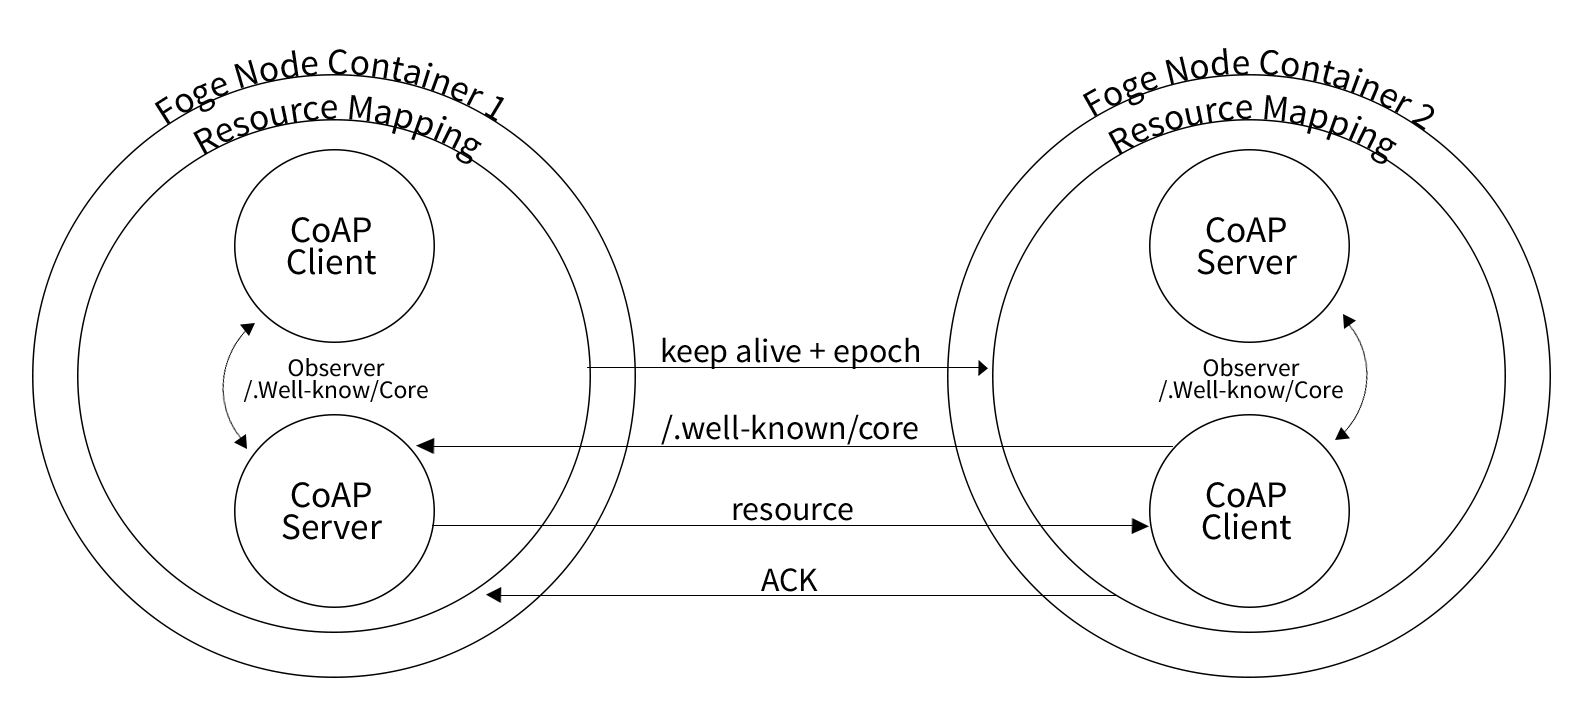
\includegraphics[width=.8\textwidth]{fig13.png}
    \caption%[This figure has a shorter caption now]%
    {\label{fig:fig13} Fog node container.}
\end{figure}


Além do protocolo de mapeamento em sí, este trabalho dispõe de uma API para o gerenciamento de recursos providos pelos CoAP servers.
Esta API possui métodos para listagem, remoção e criação de recursos e deve ser executada a partir do host que gerencia os container.
Assim, conseguimos proporcionar o dinamismo que a névoa necessita para a realização de testes no comportamento do protocolo de sincronização.



\section{Cenários de teste}
% Seção: "Cenários de teste"

% A validação deste trabalho consiste em realizar simulações que faça com que o protocolo execute suas funcionalidades de acordo com os resultados descritos na Seção anterior, sendo assim, 
% algumas situações devem ocorrer para que as validações sejam realizadas.
% Estas situações serão abordadas nos cenários de teste da Seção a seguir.


Utilizando como base a Figura \ref{fig:fig7}, e partindo do pressuposto que todos os nodos da névoa já estão com seus recursos sincronizados corretamente,
iremos exemplificar os cenários de testes elencados abaixo.

\begin{enumerate}
    \item Entrada de algum equipamento na rede e este anunciando seus recursos. 
    \item Atualização das listas globais quando algum equipamento deixar de responder as mensagens de keep alive.
    \item Atualização da lista de recursos quando algum edge device é adicionado ou removido de um nodo da névoa.
\end{enumerate}

\begin{figure}[H]
    \centering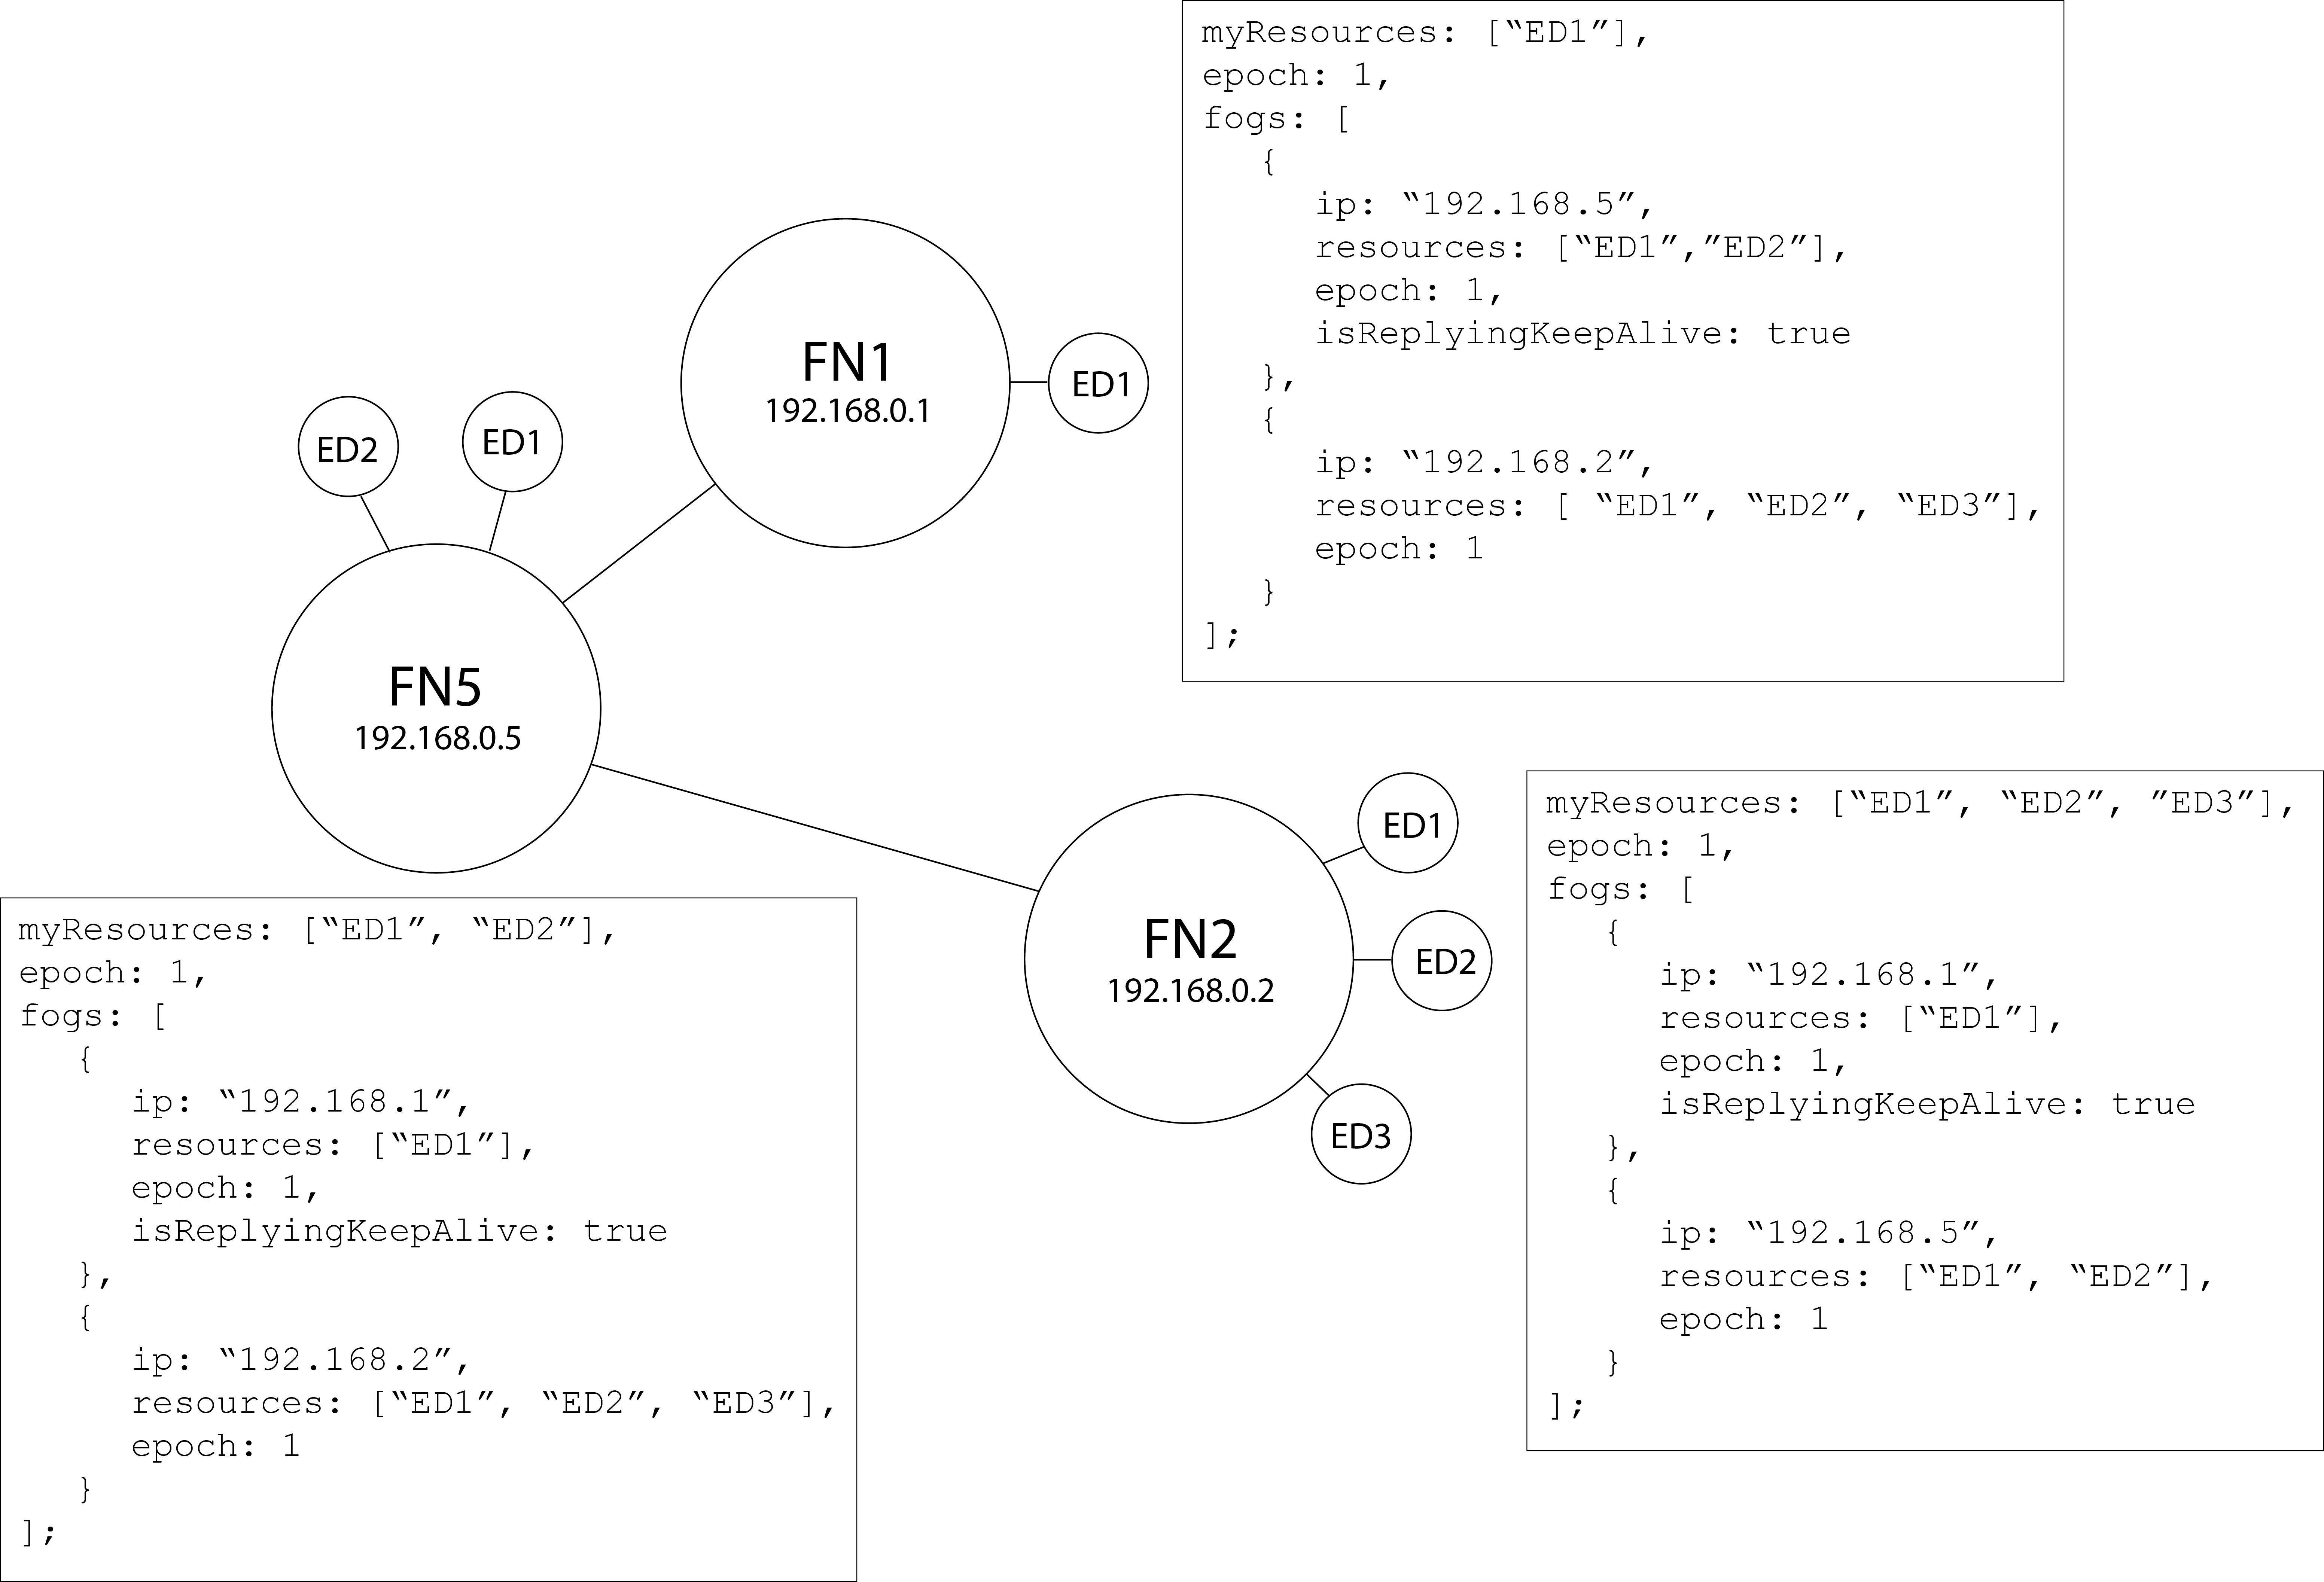
\includegraphics[width=.8\textwidth]{fig7.png}
    \caption%[This figure has a shorter caption now]%
    {\label{fig:fig7} Topologia base para cenário de teste.}
\end{figure}

O item 1 não será demonstrado agora, uma vez que as Subseções 3.2.2 e 3.2.3 já o fizeram, portanto, partiremos diretamente para o segundo item da listagem.

O segundo item trata-se de quando um nodo deixa de responder mensagens de keep alive, e a Figura \ref{fig:fig7} será utilizada para ilustrar este funcionamento.
Na Figura \ref{fig:fig8}, o nodo FN1 não respondeu, no tempo previamente estipulado, a mensagem de keep alive enviada pelo nodo FN2, 
portanto, o nodo destinatário foi marcado em FN2 como parcialmente inativo.


\begin{figure}[H]
    \centering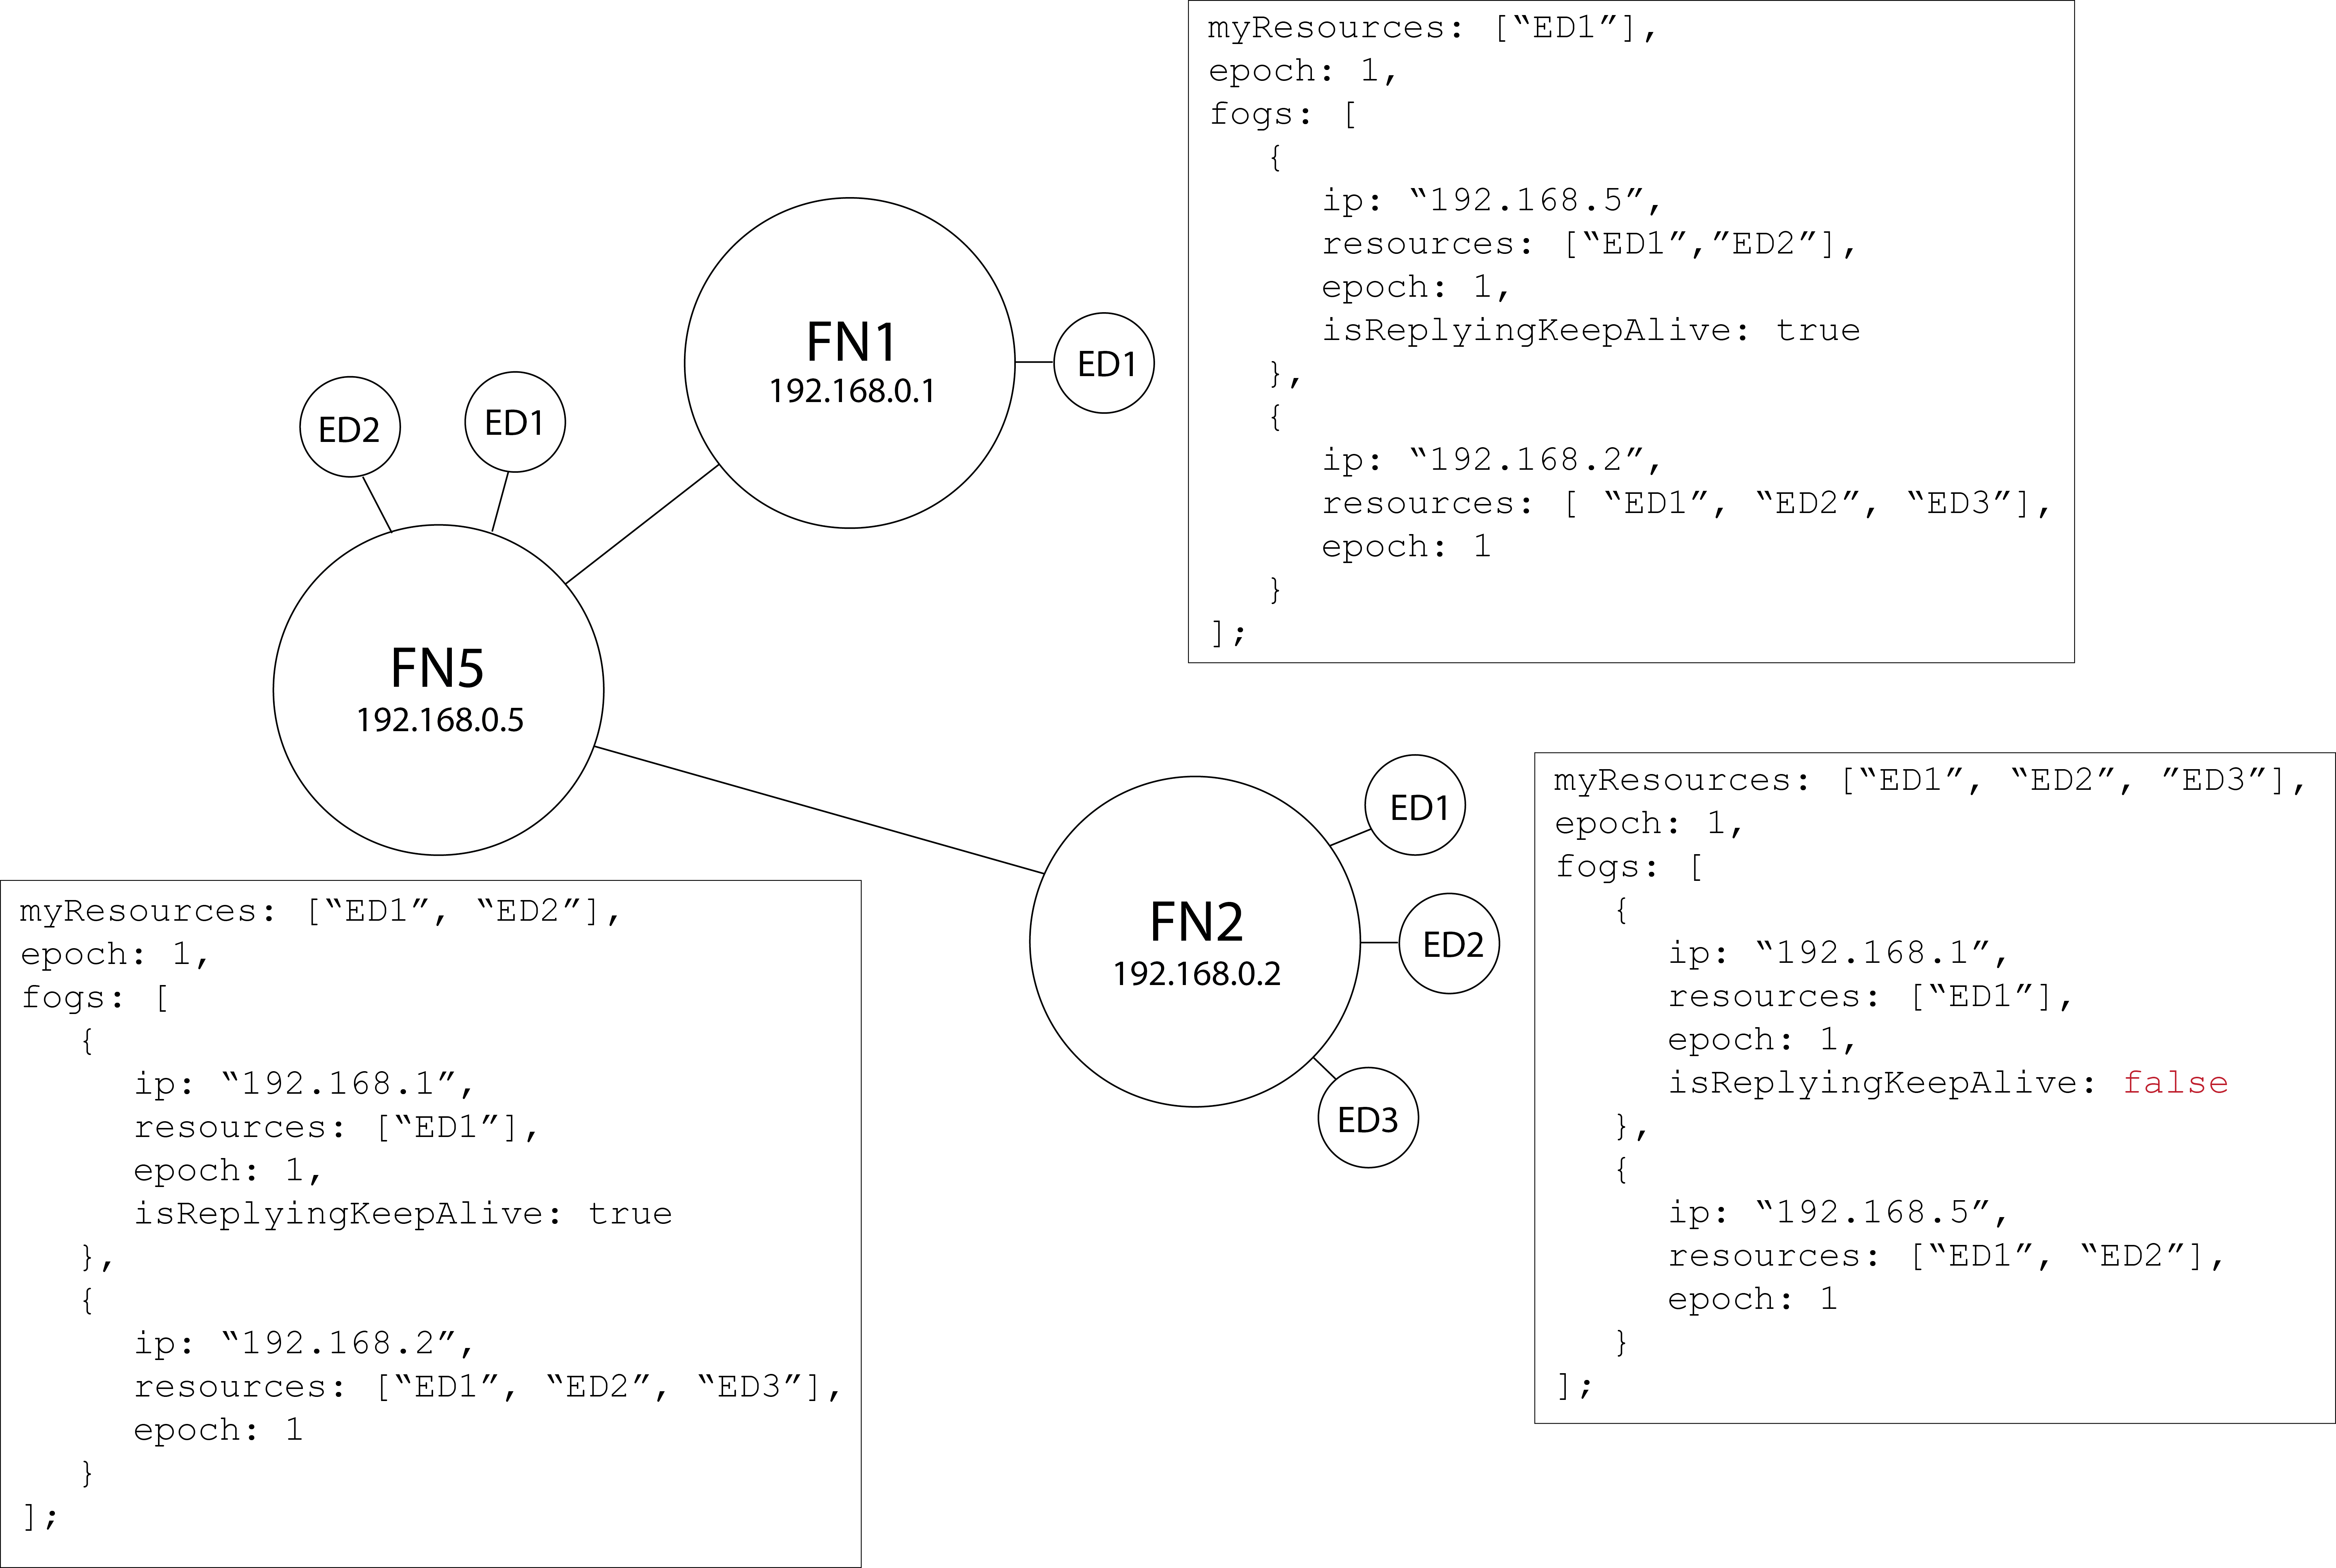
\includegraphics[width=.8\textwidth]{fig8.png}
    \caption%[This figure has a shorter caption now]%
    {\label{fig:fig8} Nodo marcado como parcialmente inativo.}
\end{figure}

Já a Figura \ref{fig:fig9} demonstra que o nodo FN1 não respondeu novamente à mensagem de keep alive enviada por FN2, por isso, foi removido de sua lista de recursos. 

\begin{figure}[h!]
    \centering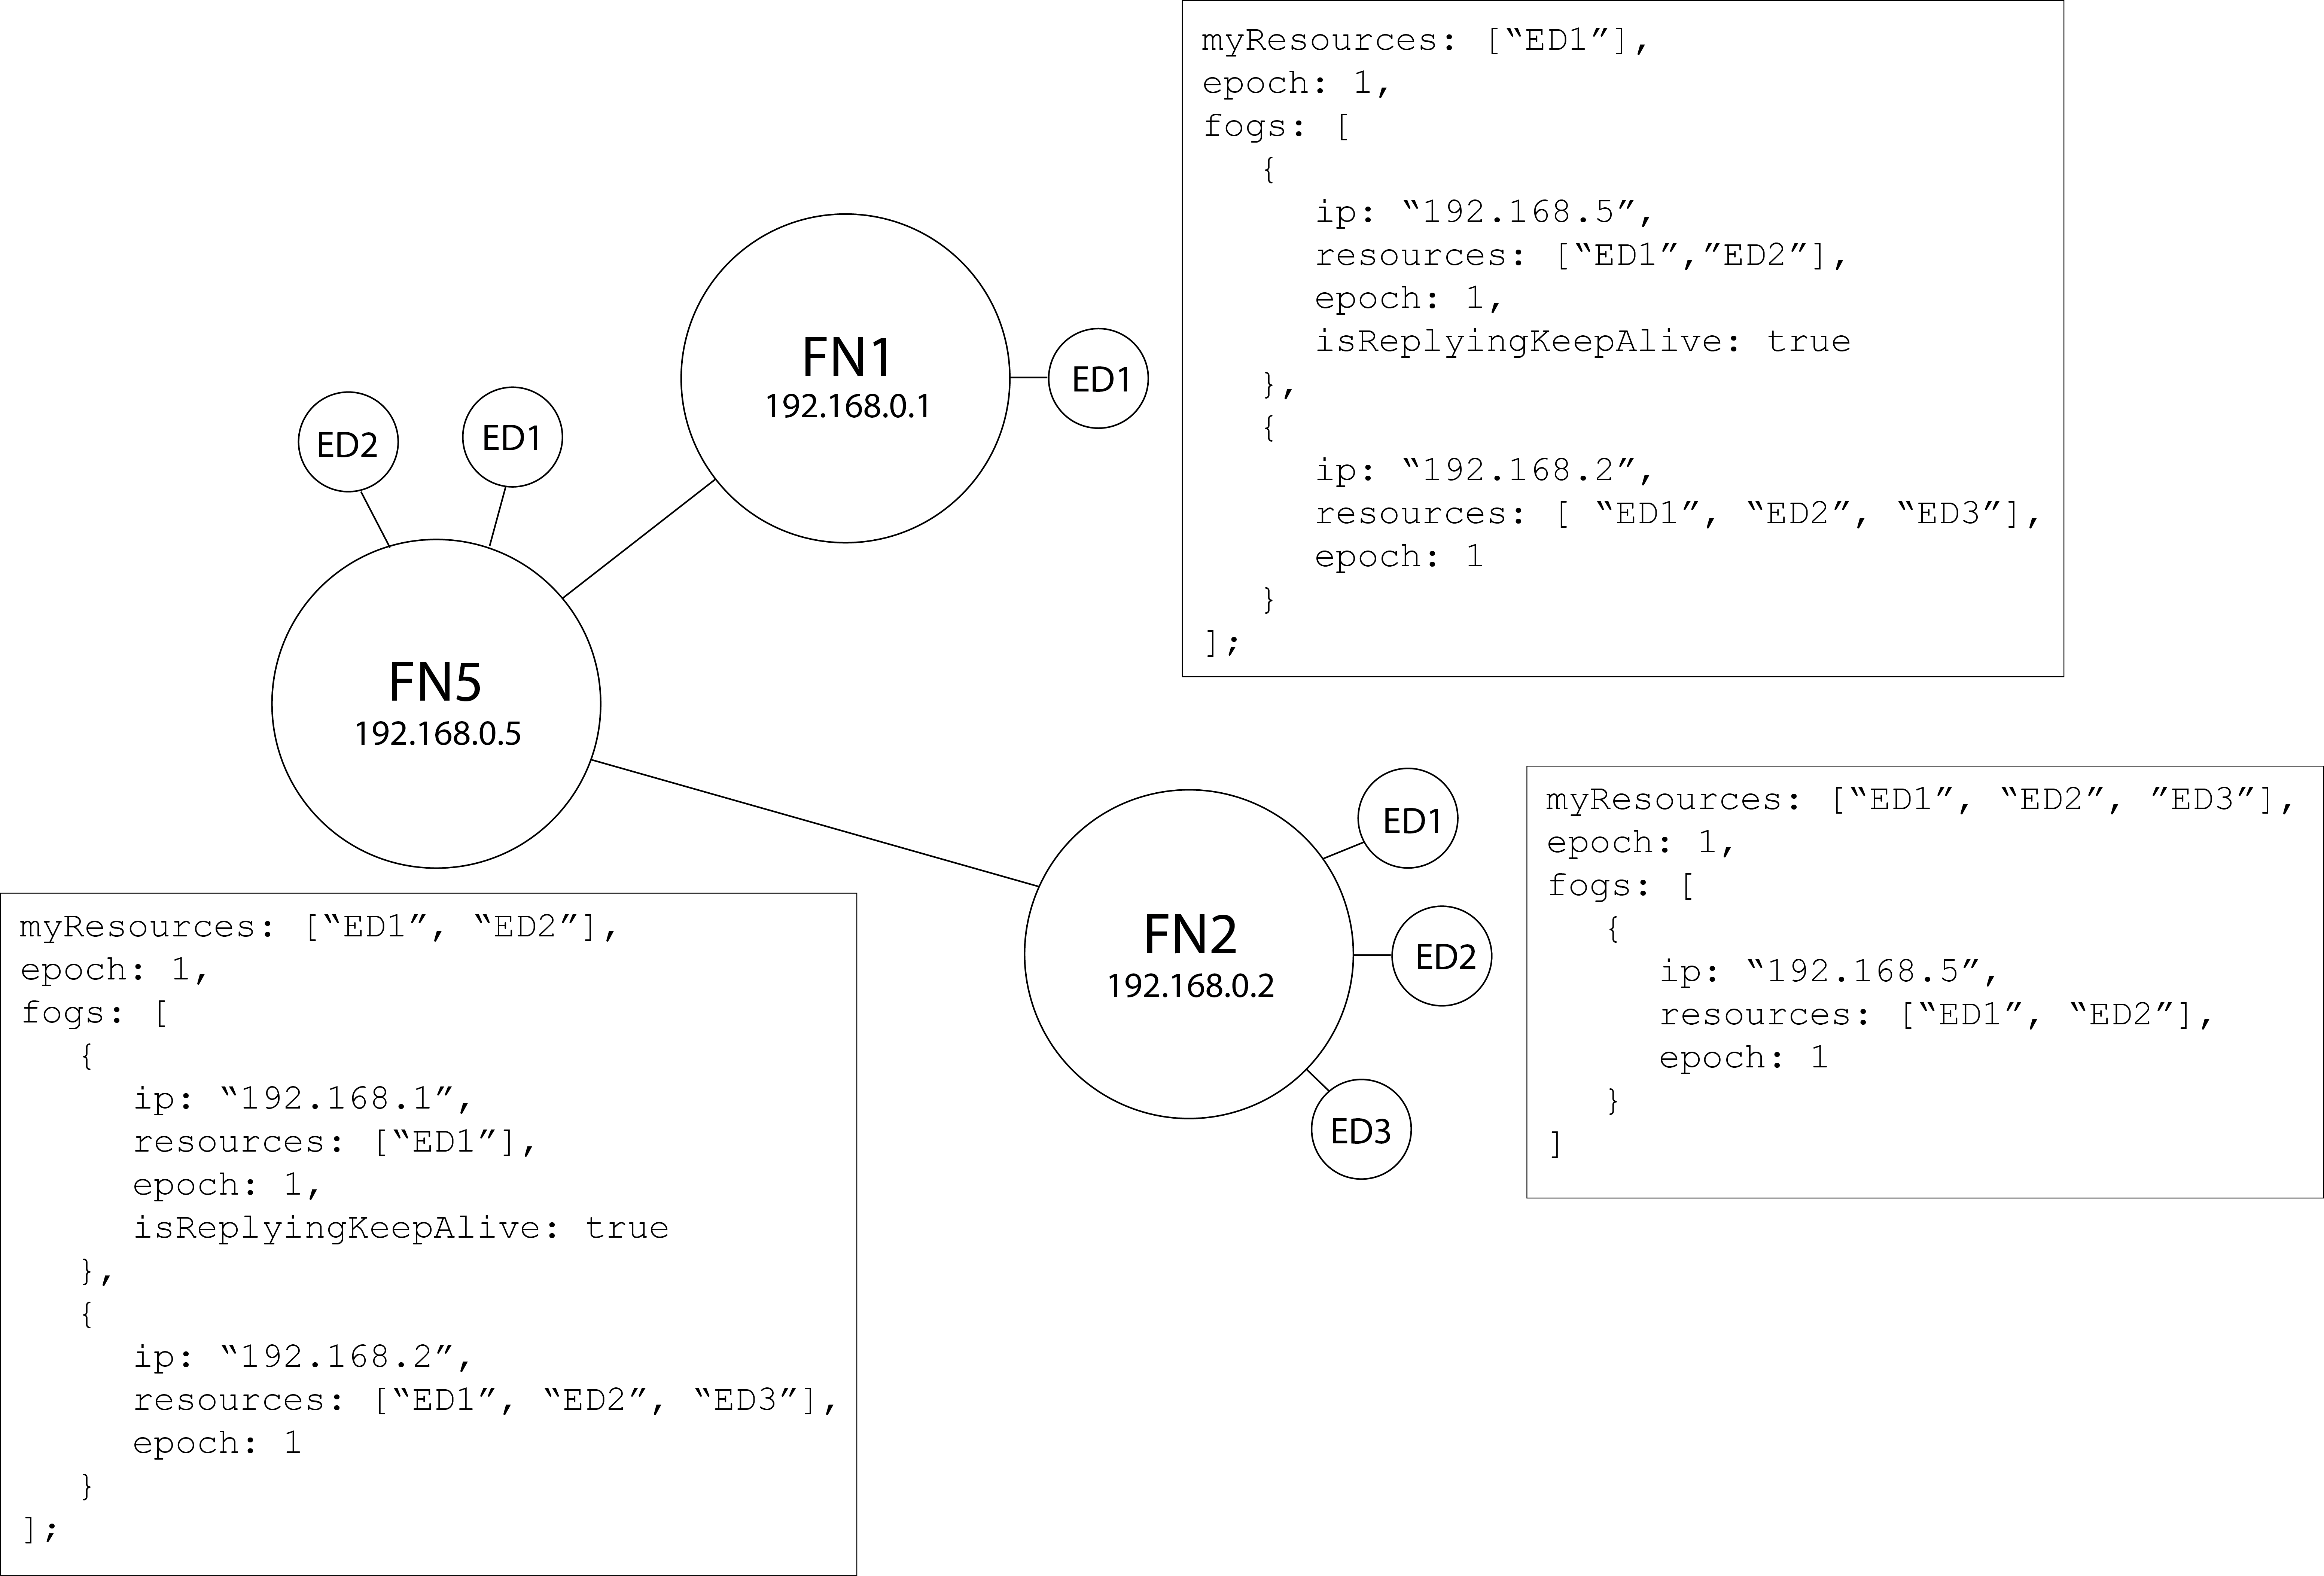
\includegraphics[width=.8\textwidth]{fig9.png}
    \caption%[This figure has a shorter caption now]%
    {\label{fig:fig9} Nodo removido da lista de recursos.}
\end{figure}

O terceiro item dos cenários de teste trata de quando o nodo está normalmente em operação, porém, um de seus recursos foi alterado, seja por incremendo de um novo edge device ou
pela remoção de um.

\begin{figure}[H]
    \centering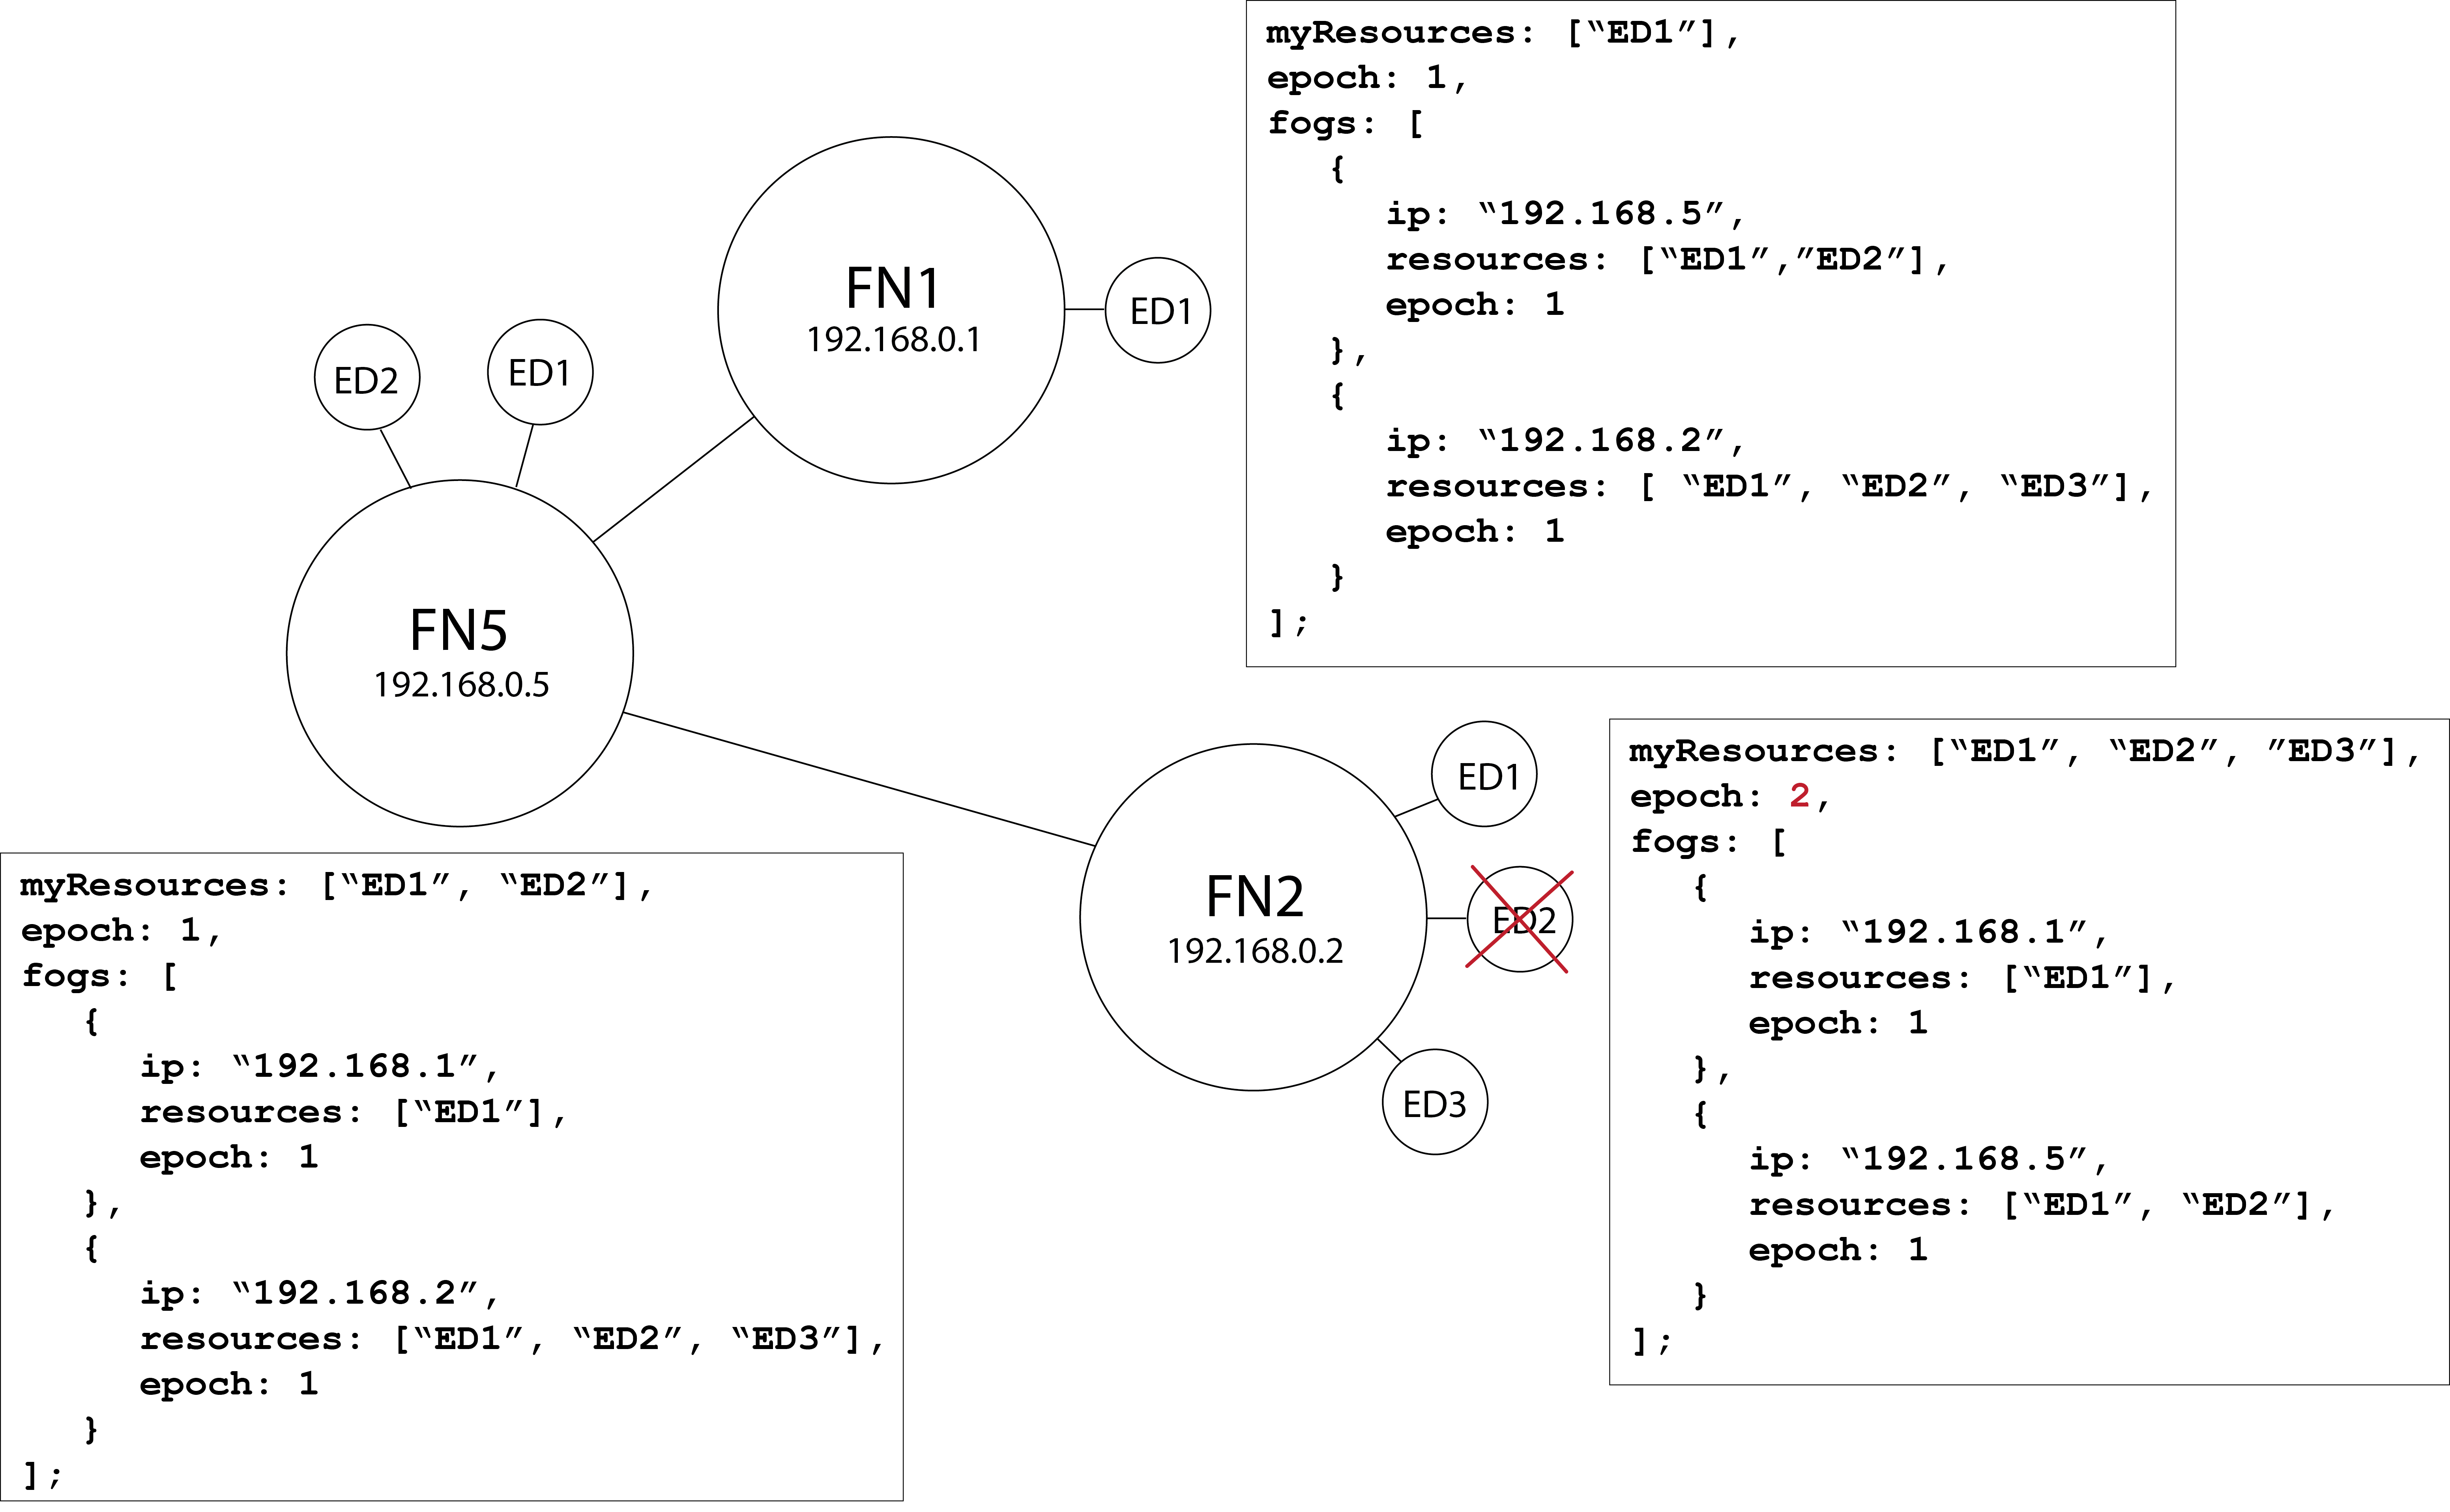
\includegraphics[width=.8\textwidth]{fig10.png} 
    \caption%[This figure has a shorter caption now]%
    {\label{fig:fig10} Edge device fora de operação.}
\end{figure}

Utilizaremos a Figura \ref{fig:fig10} como exemplo básico, e nela podemos observar que o edge device denominada ED2 vinculado ao nodo FN2 parou de funcionar.
Para este cenário, o nodo que hospeda ED2 deve estar ciente que este edge device está inoperante, e assim atualizar a sua \textit{época}.
O nodo que possui o edge device inoperante, então, terá sua época enviada juntamente com as mensagens de keep alive.
Assim, quando o nodo receber esta mensagem poderá comparar a época armazenada em sua lista de fogs com a época recebida pelo keep alive, e após a validação da divergencia realizará
um Requisição diretamente ao nodo para que possa atualizar sua lista de recursos globais.

\begin{figure}[H]
    \centering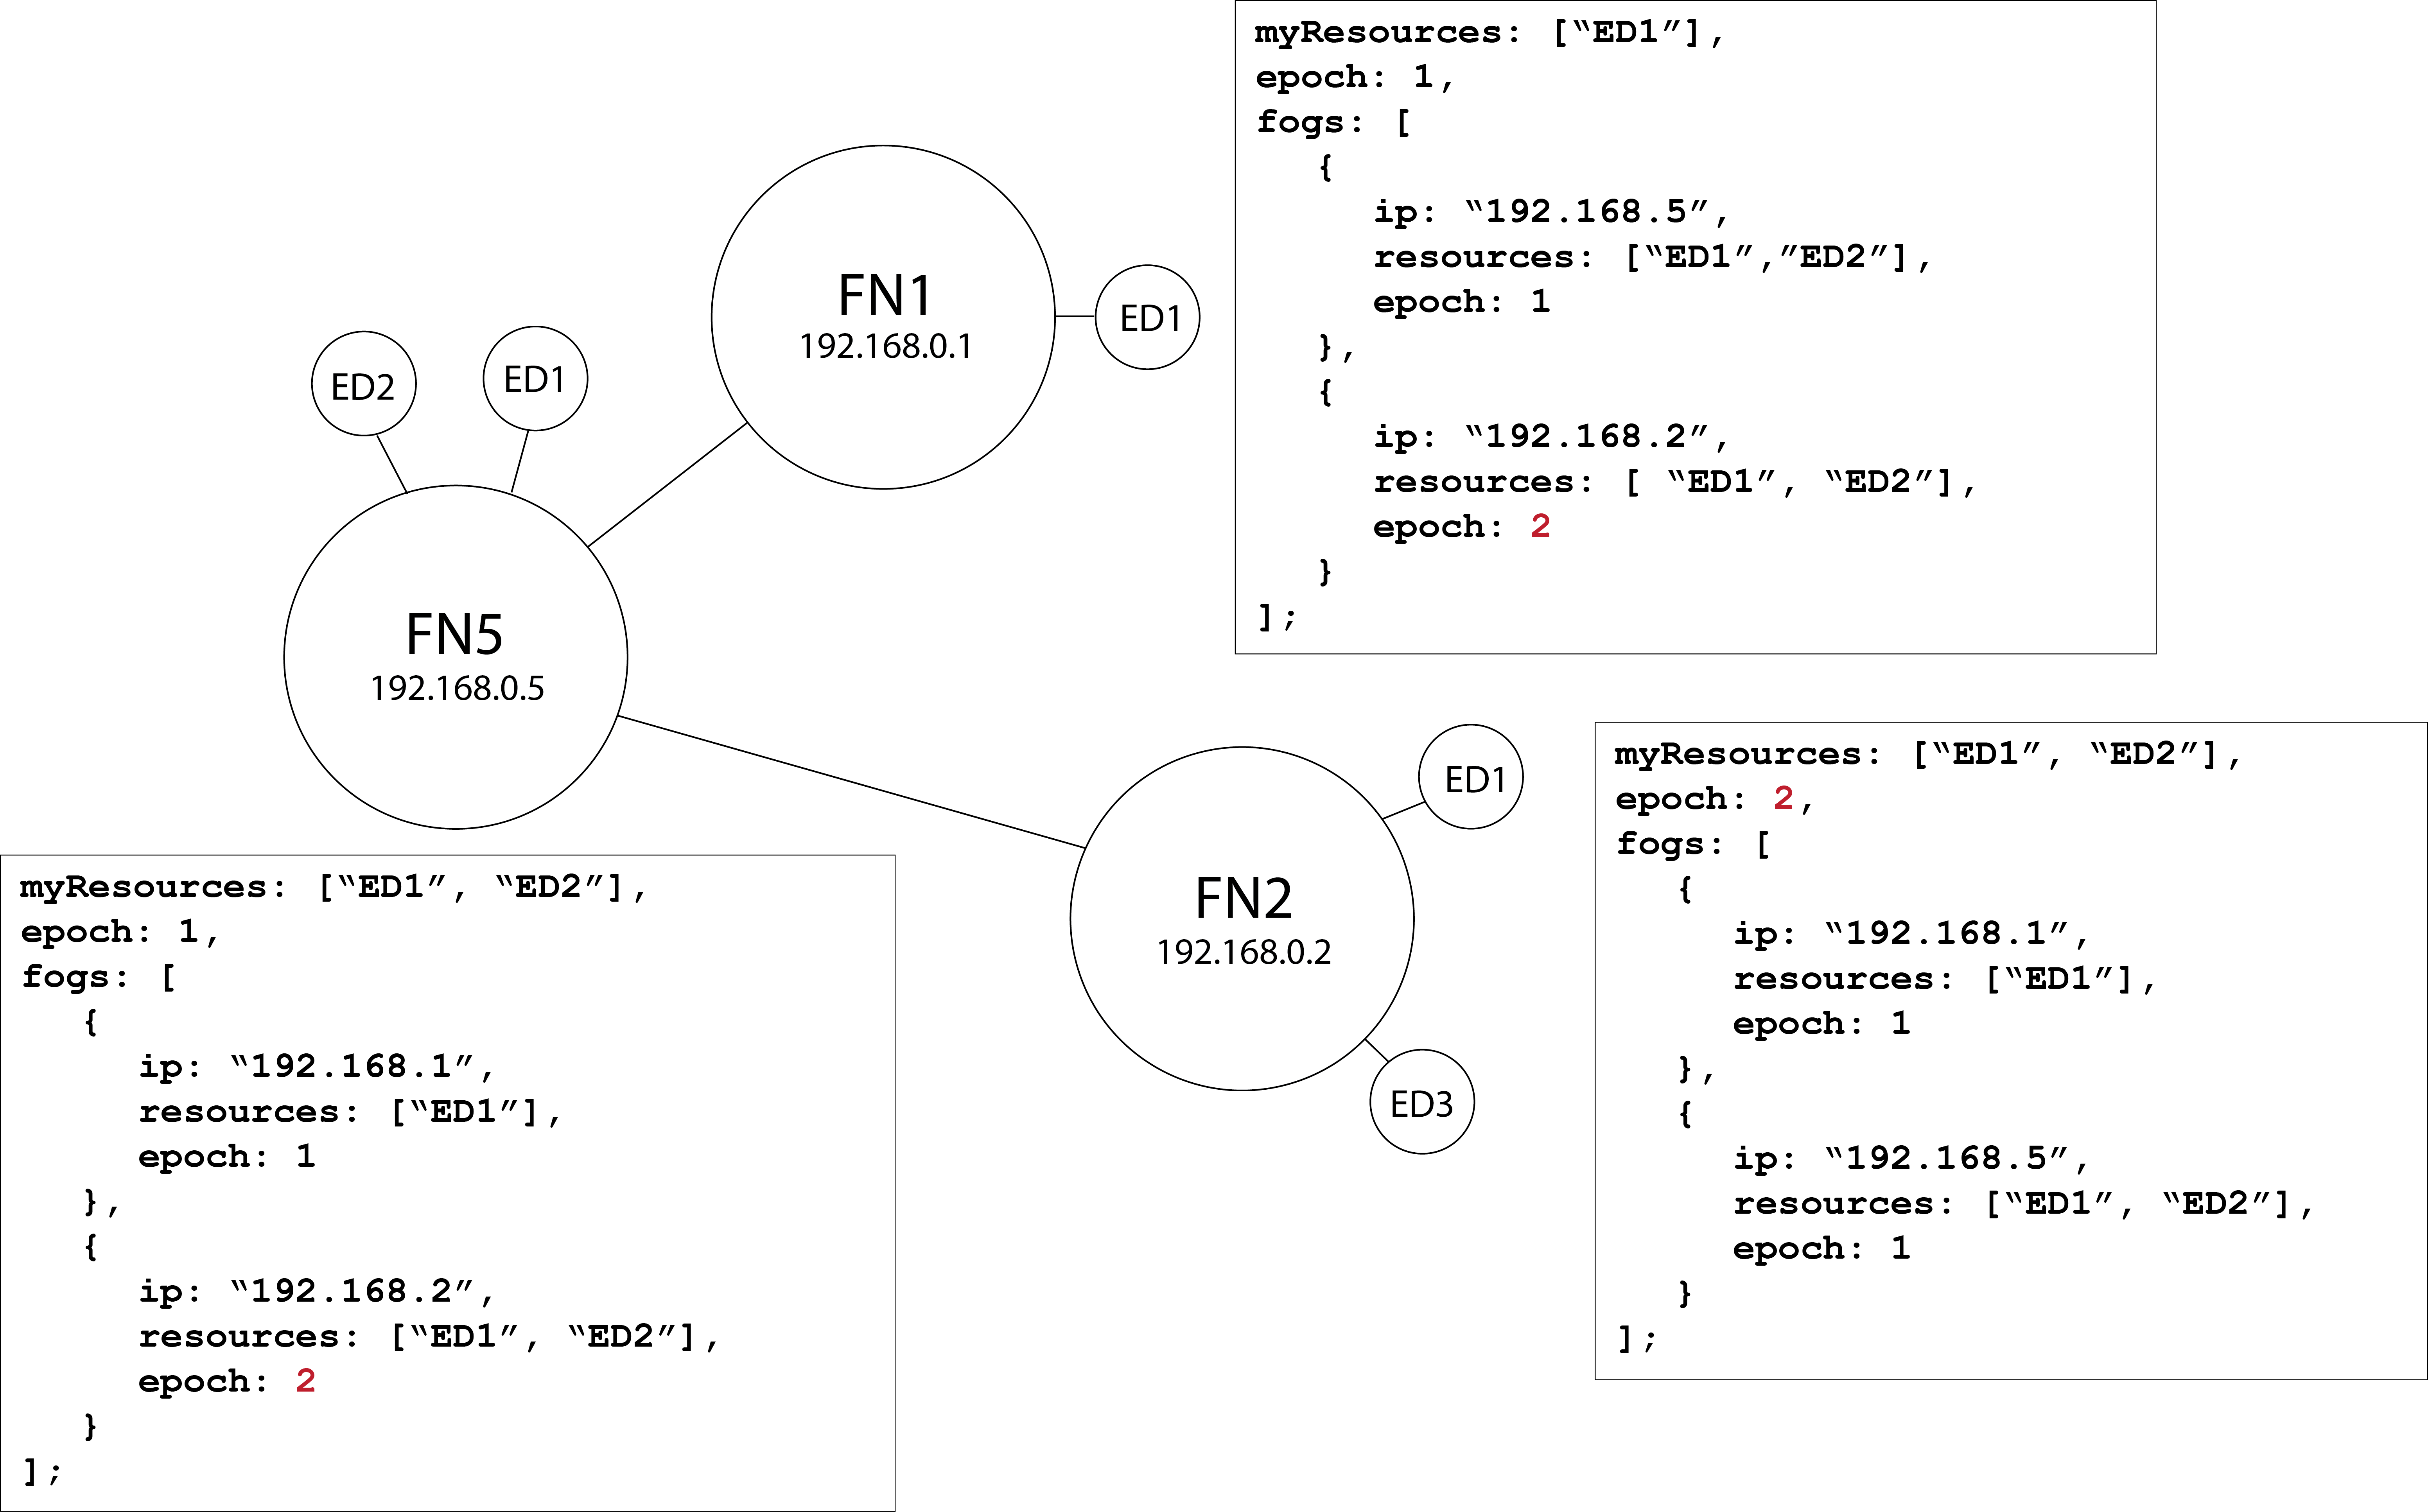
\includegraphics[width=.8\textwidth]{fig11.png} 
    \caption%[This figure has a shorter caption now]%
    {\label{fig:fig11} Estado da névoa após atualização de recursos.}
\end{figure}





\section{Estudos de caso}
% Seção: "Estudos de caso" (pelo menos 2) - pensar em alguma aplicação, onde por exemplo tens um conjunto amplo de recursos (por exemplo, diversos sensores e atuadores, luminárias, cameras, etc, tipo o prédio 32 da PUC). Pensa que os usuários de tal ambiente (alunos, professores, etc) são potenciais fornecedores de recursos (o alunos é identificado por seu smartphone na rede local e está inscrito em diversas disciplinas). Informações sobre presença (ou ausência) poderiam ser registradas, o aluno poderia ser informado sobre a sala/lab que deveria se dirigir juntamente com o tópico da aula... Sei lá! Tem que pensar em uma forma se simular, de maneira simplificada, um cenário como esse.
 %como foi feito e metodologia experimental
  %\include{cap5} %resultados e analise
  %\include{cap6} %conclusao e trabs futuros
  
  %----------------------------------------------------------------
  % Aqui vai a bibliografia. Existem 3 estilos de citação: use
  % 'tcc-alpha' para citações do tipo [Abc+] ou [XYZ] (em ordem
  % alfabética na bibliografia), 'tcc-num' para citações
  % numéricas do tipo [1], [20], etc., em ordem de referência e
  % 'tcc-alpha-full' para citações estilo 'alpha' mas com nomes completos.
  %----------------------------------------------------------------
  %\bibliographystyle{tcc-alpha-full}
  \bibliographystyle{tcc-num}
  \bibliography{bibliography}
  
  %----------------------------------------------------------------
  % Após \appendix, se iniciam os capítulos de Apêndice, com
  % numeração alfabética.
  %----------------------------------------------------------------
  % \appendix
  % \chapter{Meu primeiro apêndice}
  % \chapter{My second appendix}
  
  %----------------------------------------------------------------
  % Aqui vão os "capítulos" de anexos. Cada anexo deve
  % ser considerado um capítulo.
  %----------------------------------------------------------------
  \anexos
  \chapter{Depuração de métricas no agronegócio}
  
A fim de simplificar a demonstração, o cénario proposto contém apenas um curral e um fog node reponsavél por coletar os dados, processá-los e enviá-los a um servidor de armazenamento na nuvem.
Esse contexto está representado na Figura \ref{fig:fig17}.

Em um primeiro momento, conforme a Figura \ref{fig:fig18}, o curral está vazio, portanto, o nodo responsável pelas medições encontra-se desligado e apenas o nodo responsável 
pelo processamento das informações enconta-se em operação.

\begin{figure}[H]
  \centering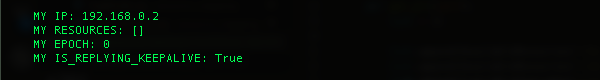
\includegraphics[width=.9\textwidth]{fig18.png}
  \caption [Fog node desligado enquanto curral permanece vazio]
  {\label{fig:fig18} Fog node desligado enquanto curral permanece vazio.}
\end{figure}

No momento em que o animal adentra o curral, o fog node e seus edge devices são ligados.
Assim, os recursos passam a fazer parte da névoa, pois suas informações são propagadas utilizando protocolo de Resource Mapping, conforme Figura \ref{fig:fig19}.
Ao sair do local de alimentação, o nodo e seus sensores são desligados e, assim, a rede volta ao estado representado pela Figura \ref{fig:fig18}.

\begin{figure}[H]
  \centering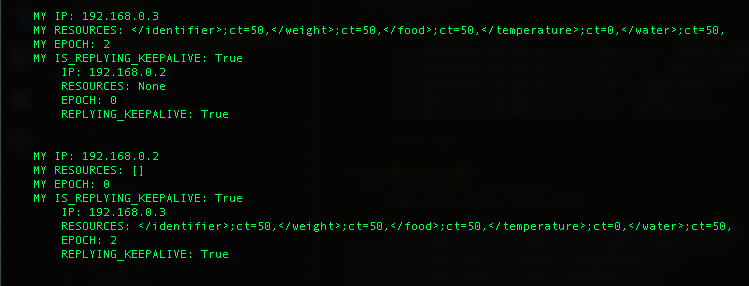
\includegraphics[width=.9\textwidth]{fig19.png}
  \caption [Fog node ligado enquanto curral permanece ocupado]
  {\label{fig:fig19} Fog node ligado enquanto curral permanece ocupado.}
\end{figure}

  
  % E aqui (para a felicidade de todos) termina o documento.
  \end{document}